\chapter{Aspects techniques}

	\section{Représentation d'un livre}
		Un livre peut contenir différentes informations. On y retrouve des items, des personnages, des paragraphes (que nous appellerons des noeuds), des choix (que nous appellerons des liens), ... Cette partie présentera la manière dont nous avons pensé ces différents éléments.

		Un livre peut contenir différentes informations. On y retrouve des items, des personnages, des paragraphes (que nous appellerons des noeuds), des choix (que nous appellerons des liens), ... Cette partie présentera la manière dont nous avons pensé ces différents éléments.

		\subsection{Représentation des noeuds}

			Nous étions d'abord parti sur une structure relativement simple pour gérer les noeuds. Ils comportaient un paragraphe, un type et une liste de choix (Voir figure \ref{fig:OldBookNode})

			\begin{figure}[H]
				\centering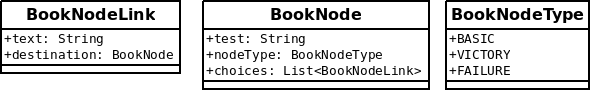
\includegraphics[width=0.70\textwidth, keepaspectratio]{img/BookNodeBefore.png}
				\caption{Ancienne représentation des noeuds}
				\label{fig:OldBookNode}
			\end{figure}

			Par la suite, nous avons voulu utiliser des classes afin de spécialiser certaines méthodes et de bien séparer les différents attributs dans différentes classes. Ainsi, seul la classe \textbf{BookNodeCombat}, représentant un noeud de combat, contient les informations sur le combat (liste d'ennemi, etc).

			Maintenant, il y a donc quatre types de noeuds représentées par différentes classes (Voir figure \ref{fig:BookNode}):

			\begin{figure}[H]
				\centering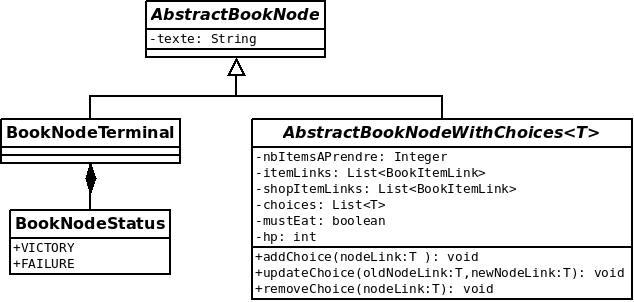
\includegraphics[width=0.90\textwidth, keepaspectratio]{img/BookNode1.png}
				\caption{Une partie de la nouvelle représentation des noeuds}
				\label{fig:BookNode}
			\end{figure}

			Tout d'abord on retrouve \textbf{AbstractBookNode} qui contient un texte correspondant aux paragraphes du noeud. En découle ensuite une deuxième classe mère \textbf{AbstractBookNodeWithChoices<T>} qui constitue la base de chaque noeud non terminal. Elle apporte diverses attributs comme la liste des items disponible sur ce noeud, le nombre d'item maximum qu'on peut en prendre, la liste des items qu'il est possible d'acheter, le nombre de points de vie perdue / gagnée sur ce noeud, mais aussi, et surtout, la liste des choix disponible. Ce dernier est défini par une List<T> car nous aurons différents type de liens et nous souhaitons qu'on noeud ne puisse posséder qu'un et un seul type de lien au sein d'une même liste.

			\begin{figure}[H]
				\centering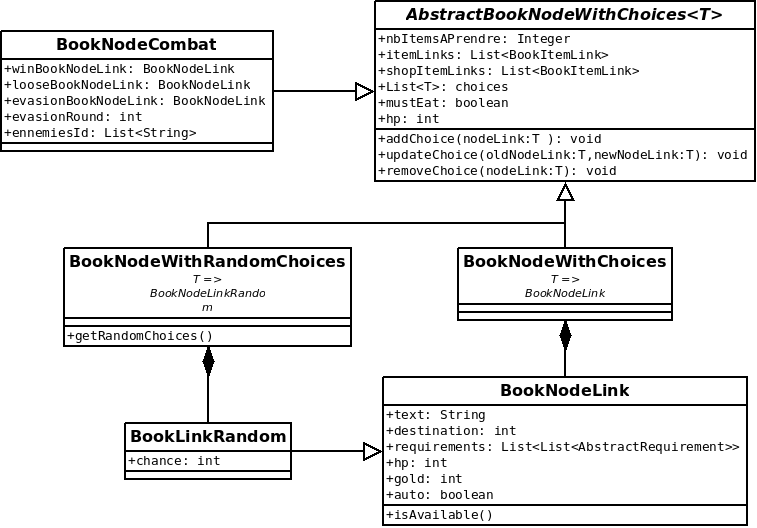
\includegraphics[width=0.90\textwidth, keepaspectratio]{img/BookNode2.png}
				\caption{L'héritage de AbstractBookNodeWithChoices<T>}
				\label{fig:BookNode}
			\end{figure}

			Parmi les classes filles instanciable, on retrouve \textbf{BookNodeWithChoices} pour les noeuds à choix simple, \textbf{BookNodeWithRandomChoices} pour les noeuds où l'on prend un choix de manière aléatoire, \textbf{BookNodeCombat} pour les noeuds de combat et \textbf{BookNodeTerminal} pour ceux de victoire et de défaite.

			\textbf{BookNodeTerminal} possède une énumération, \textbf{BookNodeStatus}, qui permet de connaître la finalité du livre, c'est à dire si le joueur à gagné ou perdu.

			Pour le \textbf{BookNodeCombat}, le choix a été fait d'ajouter trois \textbf{BookNodeLink} afin de représenter les différentes issues du combat : victoire, évasion, defaite. Cela permet donc d'avoir, au maximum, un lien possible pour chaque finalité du combat. Nous avons donc redéfini les méthodes spécifiques aux choix, c'est à dire celle pour récupérer les choix, celle pour les supprimer et celle pour les mettre à jour. La liste de la classe mère n'est plus utilisable. Il s'agit d'une grosse erreur de notre part. En effet, cette classe demande un traitement spécial à presque tous les endroits où l'on peut gérer des noeuds. Il aurait plutôt fallu ajouter les choix dans la liste parente et avoir un moyen de faire une distinction afin de savoir lequel est celui de victoire, de défaite ou d'évasion. Nous n'aurions pas eu à redéfinir autant de fois des comportements particuliers pour ce noeud avec des "instanceof". Par manque de temps et au vu des changements importants que cela nécessitait, pour faire cela proprement nous n'avons pas pu changer cela. Une liste contenant les ID des ennemis que l'on doit combattre y est également renseignée. Les ennemis peuvent ensuite être retrouvés dans le livre à l'aide de cet ID.

			Pour le \textbf{BookNodeWithRandomChoices}, la méthode \textit{getRandomChoices} a été ajoutée, afin de sélectionner un choix de manière aléatoire en fonction de la probabilité de chaque lien.

		\subsection{Représentation des liens}
			\label{sub:liens}

			Les noeuds sont liés par des liens. Ces liens sont soit définis par la classe \textbf{BookNodeLink} ou \textbf{BookNodeLinkRandom}. Pour éviter les redondances, cette dernière extends de \textbf{BookNodeLink}. Elles prennent donc toutes les deux un texte, une destination (défini par le numéro du noeud) et enfin, une liste de prérequis.

			Pour le \textbf{BookNodeLinkRandom}, la classe à besoin d'une variable pour gérer la probabilité, afin de définir la chance d'aller vers ce noeud. On comprend maintenant mieux l'utilisation de la généricité, car, si on ne le fait pas, il serait possible de mélanger des choix avec probabilité et d'autres qui n'en possède pas.

		\subsection{Représentation des personnages, items}

			Nous allons maintenant parler des personnages et des items du livre. Bien qu'il n'y ai pas grand chose à expliquer sur eux, car il s'agit de classes possédant beaucoup de "getters" et "setters", nous souhaitons détailler certains choix faits.

			Commençons par les personnages. Ceux ci sont définis par la classe \textbf{BookCharacter} dans le package magic\_book.core.game. Cette classe possède presque uniquement des "getters" et "setters" bien qu'elle possède également quelques méthodes utilitaires.

			\begin{figure}[H]
				\centering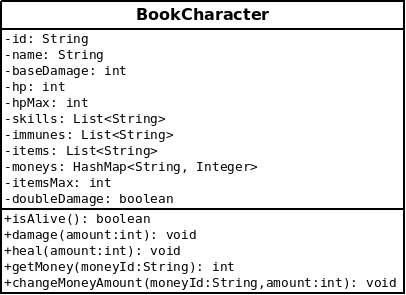
\includegraphics[width=0.45\textwidth, keepaspectratio]{img/book_character.png}
				\caption{UML sur la gestion des personnages}
			\end{figure}

			Concernant les listes de String (skills, immunes, items), il s'agit d'une liste contenant les ID. Pour "immunes", il s'agit des ID des skills contre lesquels le personnage est immunisé. Cela permet aux items et aux skills de n'être référencés qu'à un seul et même endroit, c'est à dire, dans la classe \textbf{Book}. Pour la monnaie, on a choisi d'utiliser une HashMap<String, Integer> afin de pouvoir gérer différents types de monnaie et leur montant dans une même histoire. Malheureusement, notre format de livre, et donc notre application, ne permet pour le moment pas de gérer pleinement cette fonctionnalité.

			Passons maintenant aux items. Ceux-ci possèdent une classe mère BookItem dans le package magic\_book.core.item.

			\begin{figure}[H]
				\centering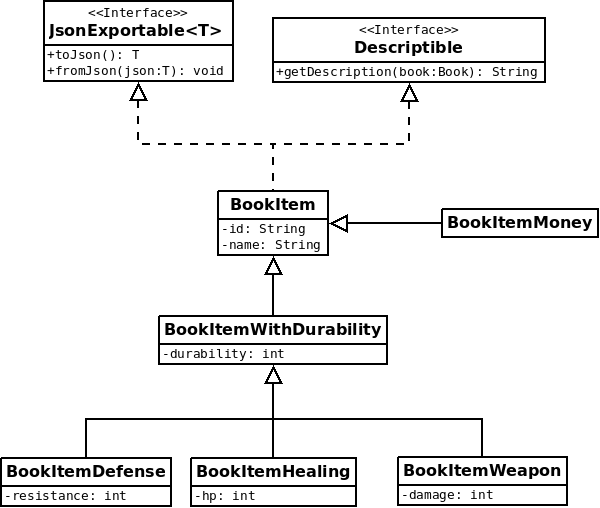
\includegraphics[width=0.66\textwidth, keepaspectratio]{img/book_item.png}
				\caption{UML sur la gestion des items}
			\end{figure}

			Avant de détailler notre choix, nous allons expliquer brièvement les deux interfaces que l'on observe. L'une se nomme \textbf{Descriptible} et permet à l'item de se décrire sous forme de String. Bien que la méthode \textit{String toString()} soit déjà prévu à cet effet, celle ci ne permet pas de prendre en argument un livre (classe \textbf{Book}). Bien entendu, c'est logique mais certains objets ont besoin du livre pour se décrire, par exemple, pour retrouver un item / personnage à partir de son id. La seconde interface, \textbf{JsonExportable} sera expliquée plus en détails dans \nameref{subsec:lecture_ecriture_fichier} à la page \pageref{subsec:lecture_ecriture_fichier}. Pour rester bref, disons qu'elle permet, la lecture et l'écriture du fichier en JSON.

			Dès lors, l'héritage prend son sens et permet une spécialisation d'un item de deux façons. La première, qui est la plus logique, permet l'ajout d'attributs spécfiques à notre classe fille. Par exemple, il serait étrange d'avoir un attribut pour savoir combien de dégât un item de type monnaie inflige. Deuxièmement, cette spécialisation intervient dans la redéfinition, par les classes filles, des méthodes des deux interfaces. En effet, chaque classe fille apporte ses propres attributs à chacune des différentes méthodes comme on peut le voir sur le listing ci-dessous. On notera l'appel à la méthode définit dans la classe mère par \textit{super.getDescription(book)} dans la méthode \textit{getDescription} , ainsi que \textit{super.toJson()} pour la méthode \textit{toJson()}.

			\begin{lstlisting}[gobble=16, language=Java, caption=Exemple de spécialisation des items]
				@Override
				public String getDescription(Book book) {
					StringBuffer buffer = new StringBuffer();

					buffer.append(super.getDescription(book));

					buffer.append("Dégats : ");
					buffer.append(damage);
					buffer.append("\n");

					return buffer.toString();
				}

				@Override
				public ItemJson toJson() {
					ItemJson itemJson = super.toJson();

					itemJson.setDamage(damage);
					itemJson.setItemType(ItemType.WEAPON);

					return itemJson;
				}
			\end{lstlisting}

		\subsection{Conditions pour accéder à un choix}

			Nous avons décidé de fournir à l'utilisateur la possibilité de définir des listes de prérequis qu'il est nécessaire de remplir afin de pouvoir accéder à un choix. Ainsi, le joueur se verra refusé l'utilisation d'un choix s'il ne possède pas un item en particulier, une certaines somme d'argent, etc.

			Les prérequis sont définis par une classe mère \textbf{AbstractRequirement}, donne lieu à une classe par type de prérequis. Chaque classe fille doit définir le comportement de la méthode \textit{boolean isSatisfied()}. Ainsi, on retrouve \textbf{RequirementItem} pour les prérequis sur la possession d'un item, \textbf{RequirementMoney} pour la posssession d'une somme d'argent ainsi que \textbf{RequirementSkill} pour la possession d'une compétence. Chacun d'entre eux possèdera donc l'id de l'élément qu'il doit vérifier, mais aussi le montant minimum nécessaire dans le cas de l'argent.

			Cependant, comment savoir si le prérequis est satisfait ? Comment connaître l'état actuel du jeu ? C'est possible grâce à la classe \textbf{BookState} qui contient toutes les informations sur l'état actuel du jeu. Nos prérequis ne portant que sur le joueur principal il est donc uniquement necessaire d'utiliser la méthode \textit{getMainCharacter}.

			Ainsi, pour savoir si un item / une compétence est possédé par personnage principal, il suffit de parcourir la liste de ceux que le personnage possède. Concernant l'argent, on récupère la somme de la monnaie possédée et on vérifie si elle correspond bien au minimum requis.

			\begin{lstlisting}[gobble=16, language=java, caption=RequirementMoney.isSatisfied(), label=lst:isSatisfied]
				public boolean isSatisfied(BookState state) {
					return state.getMainCharacter().getMoney(moneyId) >= amount;
				}
			\end{lstlisting}

			Nous avons souhaiter fournir encore plus de flexibilité à cette manière de faire, ainsi, il est possible d'avoir une liste de prérequis à satisfaire afin de pouvoir accéder au choix voulu. Il est donc maintenant possible de créer un choix qui nécessite à la fois de "posséder un pass" et "50 euros" sur soit par exemple. Là encore, nous avons décidé de fournir une possibilité supplémentaire en permettant de proposer des conditions alternatives. C'est à dire de fournir une liste de prérequis alternative capable de permettre l'accès au choix. Nous avons donc différentes liste contenant elles même des conditions qu'il est nécessaire de satisfaire en même temps. Il est donc maintenant possible de faire des conditions comme suit : ("posséder un pass" ET "50 euros") OU ("pouvoir se téléporter") OU ("posséder 50 euros" ET "posséder 50 yen").

			Ainsi, on comprend mieux le rôle de la méthode nommée \textit{isAvailable()} dans \textbf{BookNodeLink} (cf : \nameref{fig:BookNode} page \ref{fig:BookNode}). Cette méthode se charge d'indiquer si une liste satisfait tous les prérequis. Bien entendu, une seule liste suffit à rendre le choix disponible et un seul prérequis non satisfait suffit à rendre la liste non satisfaite car il s'agit du principe même des OU et des ET.


			\begin{algorithm}[H]
				\DontPrintSemicolon
				\KwIn{state : BookState}
				\KwData{
					requirements : List<List<AbstractRequirement> liste des prérequis\;
				}

				\uIf{requirements.length == 0}{
					\Return{True}\;
				}
				\;
				\For{List<AbstractRequirement> groupRequirement in requirements}{
					satisfied: bool\;
					satisfied = true\;
					\For{AbstractRequirement r in groupRequirement}{
						\uIf{not r.isSatisfied(state)}{
							satisfied = false\;
							break\;
						}
					}

					\uIf{satisfied}{
						\Return{true}
					}
				}
				\;
				\Return{false}

				\caption{Disponibilité du choix}
			\end{algorithm}

		\subsection{Prendre un choix de manière aléatoire}

			Supposons que nous souhaitons faire un paragraphe durant lequel le joueur doit passer sur un pont en bois qui semble plutôt vieux. Il serait totalement ridicule de laisser au joueur la possibilité de choisir si le pont doit céder ou non. Ce choix relève plutôt de l'ordre de l'aléatoire. Nous savons donc maintenant que pour faire cela, une instance de \textbf{BookNodeWithRandomChoices} est necessaire. Mais comment tirer un choix de manière aléatoire ?

			Pour cela, on ajoute d'abord tous les liens disponibles, c'est à dire, tous les liens où le joueur peut avoir accès en fonction des prérequis demandés. Si aucun lien n'est disponible, on retourne "null" symbolisant une erreur. Dans le cas contraire, on commence par calculer la somme des probabilités sur les noeuds disponibles. On tire ensuite un nombre aléatoire en fonction de cette somme. Enfin, il ne nous reste plus qu'à retrouver le choix correspondant en enlevant successivement la probabilité de chaque lien jusqu'à atteindre un nombre inférieur à zéro.

			\begin{lstlisting}[gobble=16, language=java, label=lst:getRandomChoices, caption=getRandomChoice()]
				List<BookNodeLinkRandom> listNodeLinkDisponible = new ArrayList();
				int somme = 0;
				int nbrChoice = 0;

				// On cherche les noeuds disponibles et on fait la somme des probabilités
				for (int i = 0 ; i < this.getChoices().size() ; i++){
					if(this.getChoices().get(i).isAvailable(state)){
						listNodeLinkDisponible.add(this.getChoices().get(i));
						somme += this.getChoices().get(i).getChance();
					}
				}

				if(listNodeLinkDisponible.isEmpty()){
					return null;
				} else {
					Random random = new Random();
					int nbrRandomChoice;
					// Si la somme des proba est à 0, on tire un noeud au hasard
					if(somme == 0) {
						nbrRandomChoice = random.nextInt(listNodeLinkDisponible.size());
						return this.getChoices().get(nbrRandomChoice);
					} else {
						nbrRandomChoice = random.nextInt(somme);
					}

					// On cherche le choix tiré
					for (int i = 0 ; i < listNodeLinkDisponible.size() ; i++){
						if(!this.getChoices().get(i).isAvailable(state)){
							continue;
						}

						nbrRandomChoice -= this.getChoices().get(i).getChance();
						if(nbrRandomChoice < 0){
							nbrChoice = i;
							break;
						}
					}
				}

				return this.getChoices().get(nbrChoice);
			\end{lstlisting}

		\subsection{La classe Book}
			\label{sub:book}

			Cette classe est la plus importante de tout le projet. En effet, c'est elle qui met en lien tous les différents éléments qu'on a pu évoquer avant. C'est en effet ce que l'on peut observer sur la figure suivante.

			\begin{figure}[H]
				\centering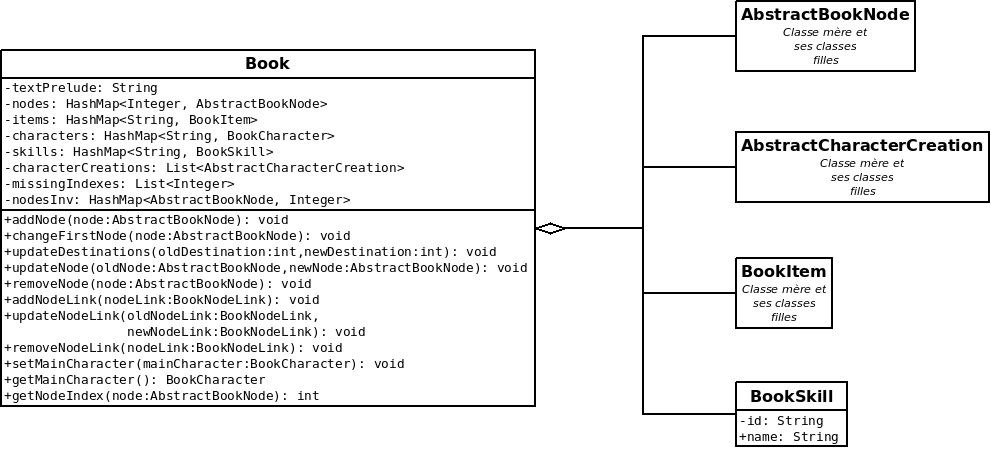
\includegraphics[width=0.8\textwidth, keepaspectratio]{img/book.png}
				\caption{UML sur la classe Book}
			\end{figure}

			Par soucis de place, les "getters" et "setters" n'ont pas été renseignés. Il en va de même pour le détail des différentes classes (\textbf{AbstractBookNode}, \textbf{BookItem}, ...). Enfin, les observateurs sont volontairement omis car ils seront détaillés un peu plus tard (dans \nameref{subsec:pattern_observer} à la page \pageref{subsec:pattern_observer}).

			Tout d'abord, commençons par expliquer comment sont sauvegardés les noeuds et les liens dans la HashMap "nodes".

			Cette HashMap possède un int comme clé, qui correspond au numéro du paragraphe. Lorsque l'on ajoute un noeud au livre, on doit d'abord lui trouver un numéro. Nous avons décidé d'établir plusieurs règles. Les paragraphes commencent à partir du numéro 1. Le numéro 1 représente \textbf{toujours} le premier paragraphe du livre. De ce fait, si l'on ajoute un noeud, il devra avoir pour numéro le 2.

			\begin{figure}[H]
				\begin{center}
					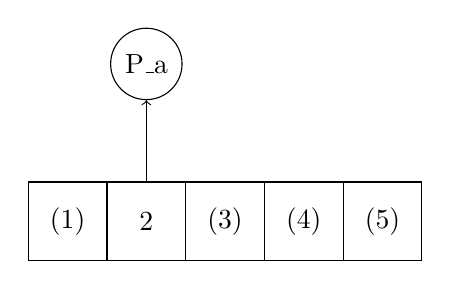
\begin{tikzpicture}
						\node[draw=black, text=black, shape=rectangle, minimum width=1cm, minimum height=1cm] (m_1) at (0,0) (1, 1) {(1)};
						\node[draw=black, text=black, shape=rectangle, minimum width=1cm, minimum height=1cm] (m_2) at (1,0) {2};
						\node[draw=black, text=black, shape=rectangle, minimum width=1cm, minimum height=1cm] (m_3) at (2,0) {(3)};
						\node[draw=black, text=black, shape=rectangle, minimum width=1cm, minimum height=1cm] (m_4) at (3,0) {(4)};
						\node[draw=black, text=black, shape=rectangle, minimum width=1cm, minimum height=1cm] (m_5) at (4,0) {(5)};

						\node[draw=black, text=black, shape=circle, minimum size=0.5cm] (p_a) at (1,2) {P\_a};

						\draw[->] (m_2.north) -- (p_a.south);
					\end{tikzpicture}
				\end{center}
				\caption{Ajout du paragraphe A}
			\end{figure}

			Les autres numéros sont représentés mais mis entre parenthèse car ils n'existent pas dans la Map. Ils sont uniquement là pour nous aider à bien visualiser ce dont on parle. Si nous décidons maintenant d'ajouter un second paragraphe alors celui-ci sera à la position 3.

			\begin{figure}[H]
				\begin{center}
					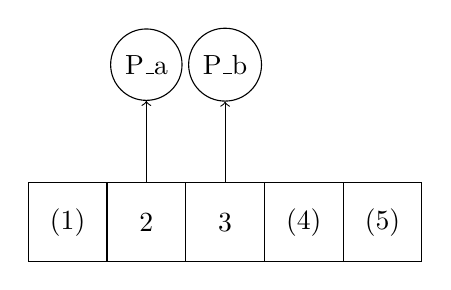
\begin{tikzpicture}
						\node[draw=black, text=black, shape=rectangle, minimum width=1cm, minimum height=1cm] (m_1) at (0,0) (1, 1) {(1)};
						\node[draw=black, text=black, shape=rectangle, minimum width=1cm, minimum height=1cm] (m_2) at (1,0) {2};
						\node[draw=black, text=black, shape=rectangle, minimum width=1cm, minimum height=1cm] (m_3) at (2,0) {3};
						\node[draw=black, text=black, shape=rectangle, minimum width=1cm, minimum height=1cm] (m_4) at (3,0) {(4)};
						\node[draw=black, text=black, shape=rectangle, minimum width=1cm, minimum height=1cm] (m_5) at (4,0) {(5)};

						\node[draw=black, text=black, shape=circle, minimum size=0.5cm] (p_a) at (1,2) {P\_a};
						\node[draw=black, text=black, shape=circle, minimum size=0.5cm] (p_b) at (2,2) {P\_b};

						\draw[->] (m_2.north) -- (p_a.south);
						\draw[->] (m_3.north) -- (p_b.south);
					\end{tikzpicture}
				\end{center}
				\caption{Ajout du paragraphe B}
			\end{figure}

			Maintenant, supposons que nous souhaitons que notre paragraphe A soit le premier noeud du livre, alors il suffira de l'ajouter dans la map l'indice 1 et de supprimer la clé 2 de notre Map.

			\begin{figure}[H]
				\begin{center}
					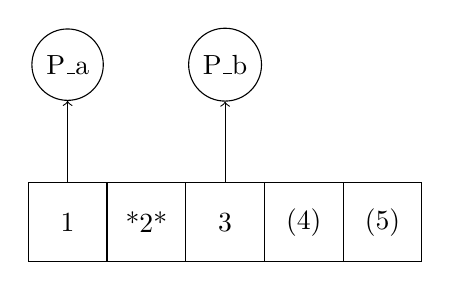
\begin{tikzpicture}
						\node[draw=black, text=black, shape=rectangle, minimum width=1cm, minimum height=1cm] (m_1) at (0,0) {1};
						\node[draw=black, text=black, shape=rectangle, minimum width=1cm, minimum height=1cm] (m_2) at (1,0) {*2*};
						\node[draw=black, text=black, shape=rectangle, minimum width=1cm, minimum height=1cm] (m_3) at (2,0) {3};
						\node[draw=black, text=black, shape=rectangle, minimum width=1cm, minimum height=1cm] (m_4) at (3,0) {(4)};
						\node[draw=black, text=black, shape=rectangle, minimum width=1cm, minimum height=1cm] (m_5) at (4,0) {(5)};

						\node[draw=black, text=black, shape=circle, minimum size=0.5cm] (p_a) at (0,2) {P\_a};
						\node[draw=black, text=black, shape=circle, minimum size=0.5cm] (p_b) at (2,2) {P\_b};

						\draw[->] (m_1.north) -- (p_a.south);
						\draw[->] (m_3.north) -- (p_b.south);
					\end{tikzpicture}
				\end{center}
				\caption{Le paragraphe A devient le noeud de départ}
			\end{figure}

			Dès lors, une case vide se retrouve disponible (symbolisé par des **). Ainsi, si l'on souhaite ajouter un noeud, il faudra d'abord combler ce vide. Le prochain paragraphe, le C donc, aura pour numéro le 2.

			\begin{figure}[H]
				\begin{center}
					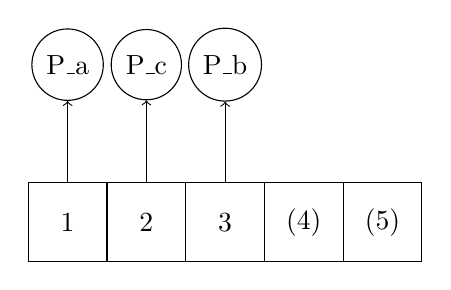
\begin{tikzpicture}
						\node[draw=black, text=black, shape=rectangle, minimum width=1cm, minimum height=1cm] (m_1) at (0,0) {1};
						\node[draw=black, text=black, shape=rectangle, minimum width=1cm, minimum height=1cm] (m_2) at (1,0) {2};
						\node[draw=black, text=black, shape=rectangle, minimum width=1cm, minimum height=1cm] (m_3) at (2,0) {3};
						\node[draw=black, text=black, shape=rectangle, minimum width=1cm, minimum height=1cm] (m_4) at (3,0) {(4)};
						\node[draw=black, text=black, shape=rectangle, minimum width=1cm, minimum height=1cm] (m_5) at (4,0) {(5)};

						\node[draw=black, text=black, shape=circle, minimum size=0.5cm] (p_a) at (0,2) {P\_a};
						\node[draw=black, text=black, shape=circle, minimum size=0.5cm] (p_b) at (2,2) {P\_b};
						\node[draw=black, text=black, shape=circle, minimum size=0.5cm] (p_c) at (1,2) {P\_c};

						\draw[->] (m_1.north) -- (p_a.south);
						\draw[->] (m_2.north) -- (p_c.south);
						\draw[->] (m_3.north) -- (p_b.south);
					\end{tikzpicture}
				\end{center}
				\caption{Ajout du paragraphe C}
			\end{figure}

			Enfin, notre application peut recommencer à ajouter des noeuds à la "fin" de notre Map.

			\begin{figure}[H]
				\begin{center}
					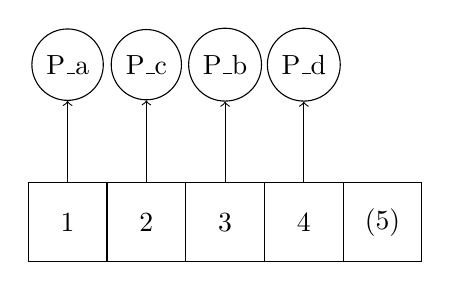
\begin{tikzpicture}
						\node[draw=black, text=black, shape=rectangle, minimum width=1cm, minimum height=1cm] (m_1) at (0,0) {1};
						\node[draw=black, text=black, shape=rectangle, minimum width=1cm, minimum height=1cm] (m_2) at (1,0) {2};
						\node[draw=black, text=black, shape=rectangle, minimum width=1cm, minimum height=1cm] (m_3) at (2,0) {3};
						\node[draw=black, text=black, shape=rectangle, minimum width=1cm, minimum height=1cm] (m_4) at (3,0) {4};
						\node[draw=black, text=black, shape=rectangle, minimum width=1cm, minimum height=1cm] (m_5) at (4,0) {(5)};

						\node[draw=black, text=black, shape=circle, minimum size=0.5cm] (p_a) at (0,2) {P\_a};
						\node[draw=black, text=black, shape=circle, minimum size=0.5cm] (p_b) at (2,2) {P\_b};
						\node[draw=black, text=black, shape=circle, minimum size=0.5cm] (p_c) at (1,2) {P\_c};
						\node[draw=black, text=black, shape=circle, minimum size=0.5cm] (p_d) at (3,2) {P\_d};

						\draw[->] (m_1.north) -- (p_a.south);
						\draw[->] (m_2.north) -- (p_c.south);
						\draw[->] (m_3.north) -- (p_b.south);
						\draw[->] (m_4.north) -- (p_d.south);
					\end{tikzpicture}
				\end{center}
				\caption{Ajout du paragraphe D}
			\end{figure}

			Voici quelques précisions supplémentaires :

			\begin{itemize}
				\item{Le principe d'indice manquant est le même pour la suppression d'un noeud}
				\item{Afin de gagner en performance pour déterminer le numéro d'un noeud déjà présent (pour savoir quel numéro sera manquant par exemple), une autre HashMap est mis à jour en même temps que celle des noeuds. Il s'agit de nodeInv. Cette map n'est rien de plus qu'une sorte de miroir pour celle des noeuds, on lui passe un noeud en clé et on obtient son numéro. Il est donc extrêmement important que les deux maps soient parfaitement identique pour éviter tout bug.}
				\item{\label{subsec:noeud_delete_missing_index}Pour déterminer l'indice d'un noeud que l'on ajoute, nous nous basons sur la taille de la Map.}
			\end{itemize}

			De ce fait, voici l'algorithme que nous avons mis en place pour l'ajout d'un noeud.

			\begin{algorithm}[H]
				\DontPrintSemicolon
				\KwIn{le noeud à ajouter : node}
				\KwData{
					nodes : Map<Integer, AbstractBookNode> liste des noeuds\;
					nodesInv : Map<AbstractBookNode, Integer> liste inversée des noeuds\;
					missingIndexes : List<Integer> liste des indices libres\;
				}

				\uIf{node in nodes}{
					\Return{}
				}

				\uIf{missingIndexes.length == 0}{
					offset: int\;
					offset $\gets$ (1 in nodes) ? 1 : 2\;
					nodes[nodes.length + offset] $\gets$ node\;
					nodesInv[node] $\gets$ nodesInv.length + offset\;
				}
				\uElse{
					nodes[missingIndexes[0]] $\gets$ node\;
					nodesInv[node] $\gets$ missingIndexes[0]\;
					missingIndexes.remove(0)\;
				}

				notifyNodeAdded(node)
				\caption{Ajout d'un noeud}
			\end{algorithm}

			La variable "offset" correspond au décalage à ajouter pour placer le noeud. Comme on commence à 2 un décalage de 2 est nécessaire. Supposons que le premier noeud est renseigné et qu'il est le seul du tableau, ajouter un nouveau noeud le placerait donc celui-ci à la position 2 + tailleDuTableau soit 2 + 1 c'est à dire 3. On a alors un décalage d'une "case". De ce fait, on doit faire un décalage de 1 uniquement si le premier noeud est renseigné.

			Voyons maintenant celui mis en place pour le changement du premier noeud.

			\begin{algorithm}[H]
				\DontPrintSemicolon
				\KwIn{le nouveau premier noeud : node}
				\KwData{
					nodes : Map<Integer, AbstractBookNode> liste des noeuds\;
					nodesInv : Map<AbstractBookNode, Integer> liste inversée des noeuds\;
					missingIndexes : List<Integer> liste des indices libres\;
				}

				\uIf{not (node in nodes)}{
					addNode(node)
				}
				\;
				updateDestinations(1, -1)\;
				\;
				indexOfNode: int\;
				indexOfNode $\gets$ nodesInv[node]\;
				\;
				oldNode: AbstractBookNode\;
				oldNode $\gets$ nodes[1]\;
				\;
				updateDestinations(indexOfNode, 1)\;
				\;
				nodes[1] $\gets$ node\;
				nodesInv[node] $\gets$ 1\;
				\;
				\uIf{oldNode != null}{
					nodes[indexOfNode] $\gets$ oldNode\;
					nodesInv[oldNode] $\gets$ indexOfNode\;

					updateDestinations(-1, indexOfNode)\;
				}
				\uElse {
					missingIndexes.add(indexOfNode)\;
					nodes.remove(indexOfNode)\;
				}

				\caption{Changement du premier noeud}
			\end{algorithm}

			\textit{NB: updateDestinations permet de changer les numéros de destination des \textbf{BookNodeLink} d'un ancien numéro, vers un nouveau}

			Si le noeud n'est pas présent dans le livre, nous commençons par l'ajouter. Les numéros des paragraphes vont êtres amenés à changer, de ce fait, il est important de mettre à jour les numéros de destination des différents liens. Nous commençons par déplacer les références du noeud 1 vers -1. En effet, cet indice n'est jamais renseigné. Ensuite, nous changeons les destinations des liens qui allaient vers le "noeud à placer en premier" pour qu'elles pointent vers le premier noeud. Nous ajoutons le noeud à cette premiere "case". Deux options sont maintenant possibles. S'il y avait déjà un premier noeud auparavant alors il faut maintenant le placer là où se trouvait l'ancien et donc, mettre à jour les liens qui vont de -1 vers ce nouvel emplacement. Si jamais il n'y avait pas de premier noeud, alors une place est maintenant manquante. On l'ajoute donc à la liste des emplacements à combler avant de pouvoir de nouveau ajouter des noeuds normalement.

		\subsection{Le pattern observer et la classe Book}
			\label{subsec:pattern_observer}

			Le pattern observer est essentiel pour la mise en place du pattern MVC. Nous avons décidé de procéder de la manière suivante :

			\begin{figure}[H]
				\centering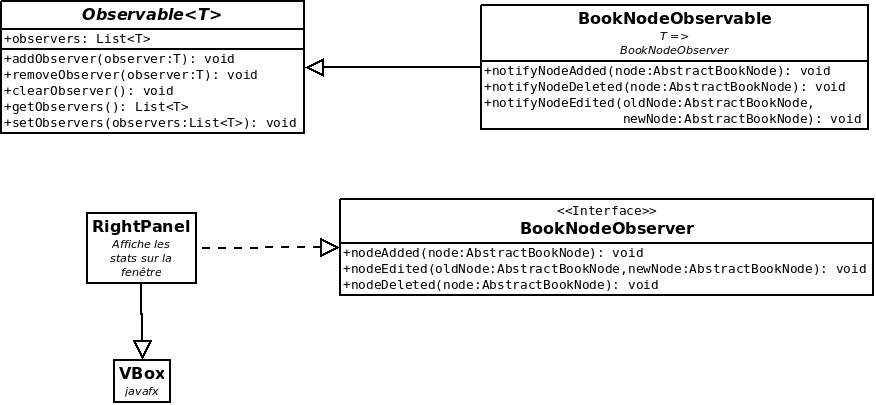
\includegraphics[width=0.8\textwidth, keepaspectratio]{img/observer.png}
				\caption{UML d'exmple sur le pattern observer}
			\end{figure}

			Comme on peut le voir, une classe mère \textbf{Observable<T>} détient une List<T> d'observers. Une méthode d'ajout, et de suppression permettent de modifier cette liste. Dès lors que l'on souhaite ajouter un nouveau type d'observer, on doit commencer par créer une nouvelle Interface avec les méthodes que l'on souhaite fournir, dans notre exemple il s'agit de nodeAdded, nodeEdited, nodeDeleted. Une fois cette interface faite, on doit alors faire une nouvelle classe \textbf{Observable}, \textbf{BookNodeObservable} dans notre cas, qui hérite de \textbf{Observable<T>}, T étant l'observer que l'on souhaite utiliser, donc \textbf{BookNodeObserver}. Ainsi, chaque Observable que l'on fera ne sera qu'une définition des méthodes pour notifier qu'un évènement s'est produit.

			Le choix à été fait de séparer les différentes parties (noeuds, liens, items, ...) du livre en différents observers afin de ne pas surcharger le nombre de méthodes à redéfinir dans les classes Observer, et donc de n'observer que ce dont on a besoin. Cependant, deux observers sont actuellement manquant, celui pour notifier d'un changement concernant le premier noeud et celui pour notifier un changement sur le personnage principal.

	\section{Lecture et écriture d'un livre}\label{sec:Json}

		L'objectif de l'application étant de concevoir un éditeur, il était important de permettre la sauvegarde et la lecture du livre que l'on édite. Le choix du format JSON est rapidement survenue. Premièrement car un fichier d'exemple qui nous a été fourni était sous ce format mais aussi car il s'agit d'une structure simple et très facile à lire. Nous avons alors utilisé GSON, une librairie, conçue par Google, extrêmement simple. Elle permet de retranscrire sous forme d'objet Java un fichier JSON structuré, c'est à dire où l'on distingue très clairement des objets qui se répète.

		Afin de lire un fichier JSON, avec cette librairie, il suffit de concevoir des objets Java avec les même attributs que ceux du fichier à lire ou à écrire. Voici un exemple très court de ce à quoi nos fichiers ressembles :

		\begin{lstlisting}[gobble=8, language=json, caption=Exemple de livre très simple, label=lst:exemple_livre]
		{
			"prelude": "Vous êtes l'enseignant qui note notre projet",
			"setup": {
				"skills": [],
				"items": [],
				"characters": [],
				"character_creation": []
			},
			"sections": {
				"1" : {
					"text": "Vous être en train d'étudier notre projet",
					"choices": [
						{
							"text": "Mettre une bonne note",
							"section": 3
						},
						{
							"text": "Mettre une mauvaise note",
							"section": 2
						}
					]
				},
				"sections": {
					"1" : {
						"text": "Vous être en train d'étudier notre projet",
						"choices": [
							{
								"text": "Mettre une bonne note",
								"section": 3
							},
							{
								"text": "Mettre une mauvaise note",
								"section": 2
							}
						]
					},
					"2": {
						"text": "Les étudiants du projet sont tristes",
						"end_type": "FAILURE"
					},
					"3": {
						"text": "Les étudiants sont satisfaits de leur travail",
						"end_type": "VICTORY"
					}
				}
			}
		}
		\end{lstlisting}

		\subsection{La structure du JSON}

		On retrouve plusieurs éléments différents. On remarque par exemple un attribut "prelude", ainsi que deux grosses parties, "setup" et "sections". Dans la suite, nous détaillerons uniquement les attributs les plus fréquemment présents.

		\subsubsection{Setup}

			Commençons par détailler "setup". Ce passage contient toutes les informations générales à notre livre. On y retrouve la liste des compétences ("skills"), la liste des items ("items") et la liste des personnages ("characters"). "character\_creation", lui, détaille toutes les étapes lors de la conception du personnage qui intervient au tout début. Celle-ci permet de sélectionner des compétences et items de départ.

			Pour le moment les compétences sont uniquement composé d'un ID et d'un nom. Dans une future \maj{} il serait intéressant d'ajouter des propriétés pour connaître la force ajoutée dans un combat, la quantité de soins à rendre par noeuds, par exemple.

			\begin{lstlisting}[gobble=12, language=json, caption=Exemple de compétence]
			{
				"id": "sixth_sense",
				"name": "Sixième sens"
			}
			\end{lstlisting}

			Les items peuvent être de différents types : KEY\_ITEM, WEAPON, DEFENSE, MONEY, HEALING. On retrouve pour tous les items un ID et un nom ("name"). Pour certains types, des attributs supplémentaires sont présents. Par exemple, un attribut "durability" peut être présent. Il permet de déterminer le nombre d'utilisation maximum d'un item. Un item de type HEALING possède un nombre de pv à rendre ("hp") tandis que ceux type WEAPON possède un montant de dégâts ("damage") par exemple.

			\begin{lstlisting}[gobble=12, language=json, caption=Exemple d'items]
			{
				"id": "backpack",
				"name": "Backpack",
				"item_type": "KEY_ITEM"
			},
			{
				"id": "healing_potion_4",
				"name": "Potion de soins (4HP)",
				"hp": 4,
				"durability": 1,
				"item_type": "HEALING"
			}
			\end{lstlisting}

			Concernant les personnages on y retrouve un ID, un nom ("name"), un nombre de pv maximum ("hp"), un boolean pour indiquer s'il a beaucoup de chance que ses coups fassent le double des dégâts ("double\_damage"), ainsi que "combat\_skill" qui représente le montant de ses dégâts.

			\begin{lstlisting}[gobble=12, language=json, caption=Exemple de personnage]
			{
				"id": "zombie_captain",
				"name": "Zombie Captain",
				"hp": 15,
				"double_damage": true,
				"combat_skill": 2
			}
			\end{lstlisting}

			Les character character\_creation peuvent être de simple texte ou de type "ITEM" ou "SKILL". On y retrouve les différents skills ou items que l'on peut prendre pour débuter notre aventure ainsi que le nombre maximum que l'on peut choisir ("amount\_to\_pick").

			\begin{lstlisting}[gobble=12, language=json, caption=Exemple de character\_creation]
			{
				"text": "Kai Disciplines\n\nOver the centuries, the Kai monks have mastered the skills of the warrior. These skills are known as the Kai Disciplines, [...]",
				"type": "SKILL",
				"skills": [
					"camouflage",
					"hunting",
					"sixth_sense",
					"tracking",
					"healing",
					"weaponskill",
					"mindshield",
					"mindblast",
					"animal_kinship",
					"mind_over_matter"
				],
				"amount_to_pick": 5
			}
			\end{lstlisting}

		\subsubsection{Sections}

			La partie "sections" est une map qui représente le numéro d'un paragraphe ainsi que le paragraphe associé. Pour rappel, il existe différents types de paragraphes : à choix, à choix aléatoire, avec des combats et terminaux. Tous possède un texte. Les noeuds terminaux possèdent un type de fin ("end\_type") afin savoir si l'on a gagné ou pas (cf : Listing \ref{lst:exemple_livre}). Les noeuds aléatoires eux, possèdent un attribut "is\_random\_pick" qui vaut "true". Pour tous les autres types de noeuds, on retrouve parmi les attributs les plus importants une liste d'items qu'il est possible de prendre, un montant d'item maximum qui peut être pris ("amount\_to\_pick") et enfin des items disponibles à l'achat ("shop").

			\begin{lstlisting}[gobble=12, language=json, caption=Exemple de paragraphe]
			{
				"text": "The back door opens [...]",
				"items": [
					{
						"id": "gold",
						"amount": 5
					},
					{
						"id": "dagger"
					},
					{
						"id": "seal_hammerdal"
					}
				],
				"amount_to_pick": 2
				"choices": [
					{
						"text": "Return to the tavern.",
						"section": "177"
					},
					{
						"text": "Study the tomb.",
						"section": "24"
					}
				]
			}
			\end{lstlisting}

			Certains paragraphes peuvent contenir un attribut "combat". Dès lors on peut connaître le choix en cas de victoire ("win"), de défaite ("loose") ou d'évasion ("evasion"). Si l'évasion est possible seulement à partir d'un certain nombre de tour on retrouve alors un attribut nommé "evasion\_round". Pour finir, un attribut "enemies" permet de connaître les personnages que l'on combat.

			\begin{lstlisting}[gobble=12, language=json, caption=Exemple de paragraphe avec des combats]
			{
				"text": "The dead zombies lie [...]",
				"combat": {
					"win": {
						"text": "If you win the combat.",
						"section": "309"
					},
					"enemies": [
						"zombie_captain"
					]
				}
			}
			\end{lstlisting}

			Pour représenter un lien vers un autre paragraphe on retrouve une liste de choix ("choices"). Ils possèdent également un texte qui correspond à l'intitulé du choix, le numéro du paragraphe suivant ("section"), un nombre d'hp à retirer, un nombre d'argent à ajouter ainsi qu'une liste de prérequis ("requirements"). Comme pour les \textbf{BookNodeLink}, il s'agit d'un tableau à deux dimensions. Le premier représente une liste de condition en OU et le second une liste de condition en ET. Enfin, pour les noeuds aléatoires, une probabilité est également présent ("weight").

			\begin{lstlisting}[gobble=12, language=json, caption=Exemple de choix]
			{
				"text": "If you have the Kai Discipline of Tracking.",
				"section": "182",
				"hp": -5,
				"requirements":  [
					[
						{
							"id": "tracking",
							"type": "SKILL"
						}
					]
				]
			}
			\end{lstlisting}

		\subsection{La lecture et l'écriture}
			\label{subsec:lecture_ecriture_fichier}

			Du fait que la structure en Json n'est pas identique à celle détaillée dans \nameref{sec:representation_livre} (page \pageref{sec:representation_livre}), nous avons fait des classes intermédiaires pour permettre cette lecture. Celles-ci sont disponibles dans le package \textit{magic\_book/core/file/json} et ne contiennent rien de plus que des "getters" et "setters". Aussi, afin de permettre une convertion entre les classes faites pour représenter un fichier json et celles faites pour être utilisées par l'application, une interface \textit{JsonExportable} existe. Celle ci permet de redéfinir 2 méthodes. L'une renvoyant la classe JSON associée à notre classe actuelle, l'autre permettant à partir d'une classe JSON d'obtenir la classe Java correspondante.

			\begin{figure}[H]
				\centering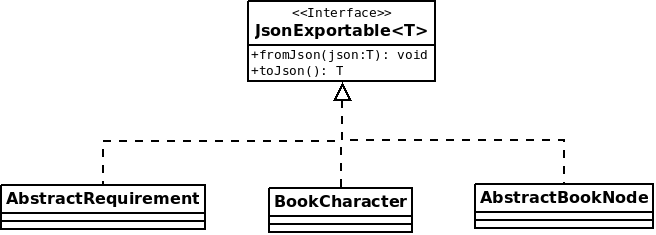
\includegraphics[width=0.66\textwidth, keepaspectratio]{img/json_exportable.png}
				\caption{L'interface JsonExportable et quelques classes qui l'implémentent}
			\end{figure}

			Enfin, les classes \textbf{BookReader} et \textbf{BookWritter} permettent de récupérer toutes les classes JSON intermédiaires pour les regrouper dans le BookJson qui correspond à la structure complète de notre livre. Ces classes sont également une couche d'abstraction à GSON car elles se chargent d'écrire le JSON correspondant dans un flux.

			Pour résumer, on peut schématiser ces échanges de telle sorte :

			\begin{figure}[H]
				\begin{center}
					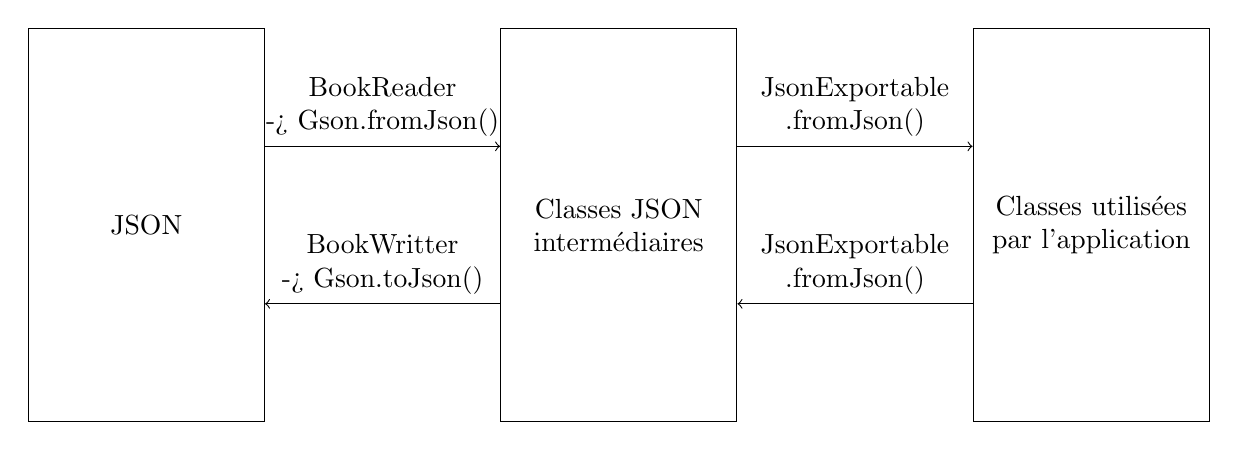
\begin{tikzpicture}
						\node[draw=black, text=black, shape=rectangle, minimum width=3cm, minimum height=5cm] (json) at (0,0) {JSON};
						\node[draw=black, text=black, shape=rectangle, minimum width=3cm, minimum height=5cm, align=center] (json_class) at (6,0) {Classes JSON\\ intermédiaires};
						\node[draw=black, text=black, shape=rectangle, minimum width=3cm, minimum height=5cm, align=center] (class) at (12,0) {Classes utilisées\\ par l'application};

						\draw[->] ([yshift=1cm]json.east) -- node[above, align=center] {BookReader\\ \fontsize{10}{12}\selectfont-> Gson.fromJson()}([yshift=1cm]json_class.west);
						\draw[->] ([yshift=-1cm]json_class.west) -- node[above, align=center] {BookWritter\\ \fontsize{10}{12}\selectfont-> Gson.toJson()}([yshift=-1cm]json.east);

						\draw[->] ([yshift=1cm]json_class.east) -- node[above, align=center] {JsonExportable\\.fromJson()}([yshift=1cm]class.west);
						\draw[->] ([yshift=-1cm]class.west) -- node[above, align=center] {JsonExportable\\.fromJson()}([yshift=-1cm]json_class.east);
					\end{tikzpicture}
				\end{center}
				\caption{Échanges pour la lecture / écriture}
			\end{figure}

	\section{Edition graphique d'un livre}

		\subsection{La fenêtre principale}

			Notre fenêtre principale est définit par la classe la MainWindow est notre fenêtre principale. Elle contient un Menu permettant de réaliser plusieurs actions (ouvrir et sauvegarder un fichier, exporter le livre, jouer, estimer la difficulté, ...) ainsi que trois zones différentes, divisées en trois autres classes.

			\begin{figure}[H]
				\centering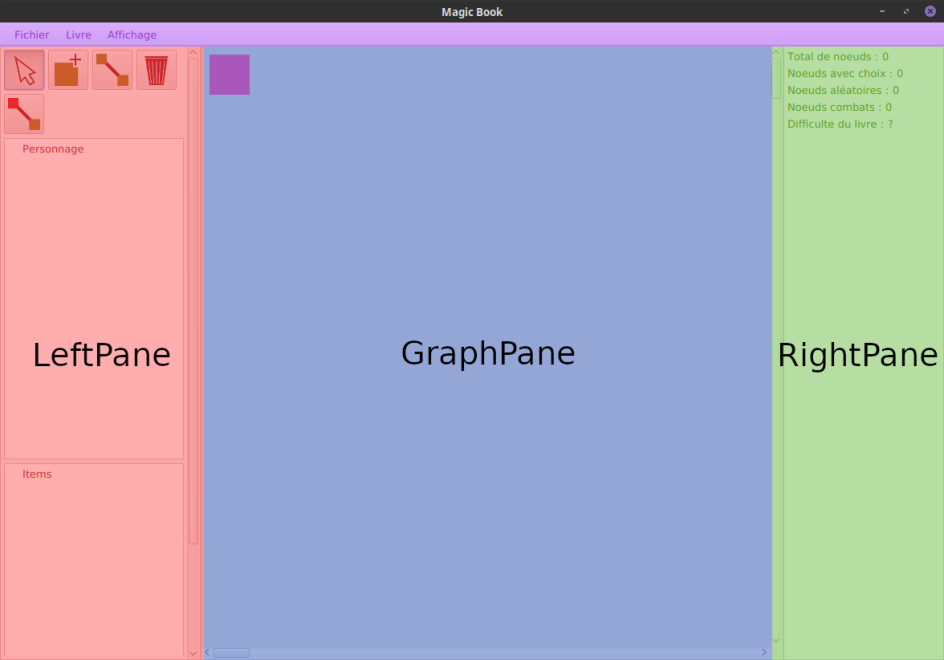
\includegraphics[width=0.50\textwidth]{img/mainwindow.png}
				\caption{MainWindow}
				\label{fig:MainWindow}
			\end{figure}

			La partie de gauche est représentée par la classe \textbf{LeftPane}. Celle-ci est composée de différent boutons permettant de changer de mode, d'une liste d'items, de personnage, de compétences constituant le livre. De l'autre côté, à droite, on retrouve une instance de \textbf{RightPane}. Cette partie permet d'afficher les statistiques du livre comme par exemple, le nombre de noeud ainsi que l'estimation de la difficulté du livre, etc. Enfin, la partie centrale défini par le \textbf{GraphPane} permet d'éditer sous forme graphique le livre. Ces trois parties utilisent le Pattern MVC ce qui leur permet également d'être réactif aux changements du livre notamment grace au Pattern Observer fournis par celui-ci (cf : \nameref{subsec:pattern_observer} page \pageref{subsec:pattern_observer}) .

			\subsubsection{Ouverture et sauvegarde du livre}

				Avant de démarrer, il faut préciser qu'une variable \textit{path} est présente dans \textbf{MainWindow} et permet de sauvegarder le fichier actuellement ouvert dans l'éditeur. Celle-ci vaut null lorsqu'aucun fichier ne l'est. C'est donc sa valeur au lancement de l'application.

				L'utilisateur peut démarrer un nouveau livre, à l'aide du menu, en cliquant sur \underline{Fichier -> Nouveau}. La classe \textbf{MainWindow} fait alors une nouvelle instance de la classe Book puis appelle sa méthode \textit{void setBook(Book)} qui se chargera de transmettre à tous les panels (LeftPane, GraphPane, RightPane) le nouveau livre. Les panels propageront alors le livre aux différents éléments qui pourraient en avoir besoin (tel que les listes d'items, de personnages, ...). Enfin, la variable \textit{path} est mise à null.

				Il est possible d'ouvrir un livre à l'aide du menu \underline{Fichier -> Ouvrir}. Une boite de dialogue s'affiche alors afin de sélectionner le livre que l'on souahite éditer. Si un livre a bien été sélectioné, alors, \textbf{BookReader} sera appellé afin de le lire (cf : \nameref{subsec:lecture_ecriture_fichier} page \pageref{subsec:lecture_ecriture_fichier}). Si le fichier est invalide, au niveau de la structure du JSON, une erreur s'affiche et le processus d'ouverture s'en arrêtera là. Une fois de plus, la méthode \textit{void setBook(Book)} de \textbf{MainWindow} est appelé afin de transmettre le nouveau livre. Enfin, si l'on a put faire toutes ces actions sans aucun soucis, la variable \textit{path} retient le chemin vers le fichier ouvert.

				Enfin, il est possible grâce à \underline{Fichier -> Enregistrer} ainsi que \underline{Fichier -> Enregistrer sous} d'enregistrer les changements sur le fichier. La sauvegarde d'un fichier se déroule comme suit ; On commence par vérifier si un fichier est déjà ouvert, grace à \textit{path}. Si ce n'est pas le cas, alors on affiche une fenêtre afin de sélectionner l'emplacement de sauvegarde. Si l'utilisateur valide son choix, alors on doit changer la valeur de \textit{path} pour enregistrer cet emplacement. On fera ensuite appel à la classe \textbf{BookWritter} pour sauvegarder le livre au format JSON (cf : \nameref{subsec:lecture_ecriture_fichier} page \pageref{subsec:lecture_ecriture_fichier}). Cependant, il existe une différence entre \underline{Fichier -> Enregistrer} et \underline{Fichier -> Enregistrer sous}. En effet, l'étape de la vérification "du fichier déjà ouvert" ne se fait que pour pour le premier des deux tandis que l'autre affichera donc toujours la fenêtre de sauvegarde peut importe la valeur de \textit{path}.

		\subsection{LeftPane}

			\subsubsection{Sélection du mode}

				Comme mentionné auparavent, ce panel contient plusieurs bouttons cliquable en haut afin de sélectionner le mode d'édition. Pour celà, nous avons utilisé des \textbf{ToggleButton}, lesquels sélectionnent l'un des 5 modes disponibles par l'énumération \textbf{Mode} à savoir : SELECT, ADD\_NODE, ADD\_NODE\_LINK, DELETE, FIRST\_NODE. Ces bouttons faisant stritement la même chose, ils sont tous créé à partir de la méthode \textit{ToggleButton createToggleButton(String, Mode)}. Cette méthode prend en paramètre le chemin vers une image ainsi que le mode que l'on souhaite sélectionner lorsque l'on clique dessus, mode qui sera appliqué au \textbf{GraphPane}. Afin de ne sélectionner qu'un seul \textbf{ToggleButton} à la fois, tous, sont contenu dans un seul et même \textbf{ToggleGroup} qui se chargera lui même de déselectionner le ToggleButton précédemment sélectionné.

			\subsubsection{Gestion des éléments du livre}

				En dessous des bouttons pour sélectionner le mode, nous retrouvons trois listes permettant chacune la gestion d'un des éléments du livre, c'est à dire, des personnages, des items et des compétences.

				Bien qu'il s'agisse d'un arbre, au vue du fait qu'ils héritent de \textbf{TreeView<T>}, nous avons fait un affichage qui correspond plus à celui d'une liste. Pourquoi ce choix ? Nous aurions voulu pouvoir par la suite organiser cette vue de manière à ce qu'elle puisse contenir différentes catégories tel que, pour les items par exemple, Autre, Arme, Défense, (...) corresondant aux différents types d'items possibles. Chaque catégorie contiendrait alors les items correspondant à ce type. Ainsi, l'UML de ces classes ressemble à celui ci :

				\begin{figure}[H]
					\centering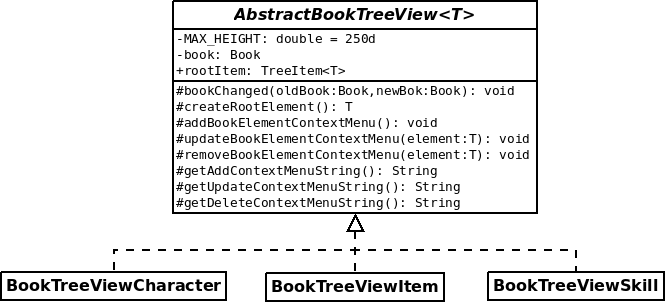
\includegraphics[width=0.7\textwidth]{img/fenetreTreeView.png}
					\caption{UML des TreeView}
					\label{fig:fenetreTreeView}
				\end{figure}

				Comme on pouvait s'en douter, chacune de ces liste hérite de d'une classe mère, \textbf{AbstractBookTreeView<T>}, permettant de gérer les comportement en commun. L'utilisation de la généricité permet de définir le type d'élément que la liste se chargera de gérer. Détaillons maintenant les différentes méthodess à redéfinir.

				Comme pour tous les autres éléments graphique, les listes sont conçue en utilisant le Pattern MVC et donc également, le Pattern Observer. De ce fait, ils réagissent automatiquement à un changement sur l'éléments qu'ils permettent de gérer (items, personnages, compétences).

				La méthode \textit{void setBook(Book)}, permet comme pour tous les autres éléments, de changer le livre actuel. Cependant des actions supplémentaires étaient requisent par les listes afin nottament de ne plus écouter les évènements sur l'ancien livre ainsi que d'afficher les éléments concernant le nouveau. Nous avons donc conçu la méthode \textit{void bookChanged(Book, Book)} qui est automatiquement appelée par \textit{void setBook(Book)} et permet à la liste d'éffectuer ces changements. Nous avons préféré fonctionner de cette manière plutôt que d'utiliser \textit{super} car cela oblige à fournir un comportement pour cette méthode et évite également l'oubli de la redéfinition de \textit{void setBook(Book)} pour traiter correctement le livre et réaliser les actions précédemment évoquées. La méthode \textit{T createRootElement()} quant a elle, permet de créer l'élément servira de label dans le TreeItem. La seul vrai valeur que l'on doit y renseigner est le nom de l'élément, les autres valeurs peuvent valoir null car elles ne seront pas utilisées. Les méthodes \textit{void addBookElementContextMenu()}, \textit{void updateBookElementContextMenu(T)}, \textit{void removeBookElementContextMenu(T)} correspondent aux actions à exécuter lorsque l'on clique sur l'action ajouter, modifier ou supprimer du menu lors d'un clique droit sur la liste. Enfin, les méthodes \textit{String getXXXContextMenuString()} permettent de récupérer le texte qui sera affiché dans le menu qui vient d'être évoqué.

		\subsection{GraphPane}
			\label{sub:GraphPane}

			Le GraphPane correspond à la zone d'édition. Elle contient des méthodes permettant l'ajout de lien ainsi que l'ajout de noeud. C'est ici que le mode va prendre tout son sens et toute son importance. En efffet, un clique sur cette partie de l'application n'aura pas les même effets selon que l'on soit en mode "ADD\_NODE" ou "DELETE".

			\subsubsection{Représentation graphique des éléments}

				Notre application ayant besoin de rerprésenter dans la fenêtre les différents élements tel que le prélude, les noeuds et les liens entre eux, voici la manière dont nous avons procédé.

				Commençons par analyser le diagramme montrant l'architecture pour les noeuds :

				\begin{figure}[H]
					\centering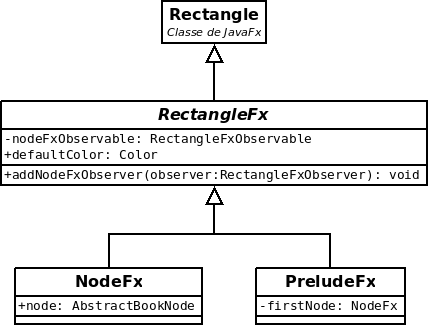
\includegraphics[width=0.6\textwidth, keepaspectratio]{img/NodeFx.png}
					\caption{UML sur la représentation des noeuds}
				\end{figure}

				Nous avons décidé de fournir un wrapper à la classe \textbf{AbstractBookNode} afin de les représenter. Nous avons appellé cette classe \textbf{NodeFx}. Celle-ci hérite de \textbf{Rectangle} qui est fournis par JavaFx. Afin d'éditer les différents éléments du livre il est également nécessaire de fournir un élément visuel représentant le départ du livre et permettant d'éditer les éléments tels que le prélude, le personnage principal, etc. Ceci est possible grace à \textbf{PreludeFx}. Les deux classes ayant des éléments en commun (une couleur et des observers, lesquels seront détaillé après), nous avons donc décidé d'ajouter une "couche" supplémentaire entre \textbf{Rectangle} et nos deux classses. C'est ce à quoi sert \textbf{RectangleFx}. Chacune des classes filles possède en attribut les éléments qu'elle à besoin, c'est à dire, le noeud représenté pour \textbf{NodeFx} tandis que \textbf{PreludeFx} a besoin, elle, du premier noeud du livre.

				Passons maintenant à la représentation des liens :

				\begin{figure}[H]
					\centering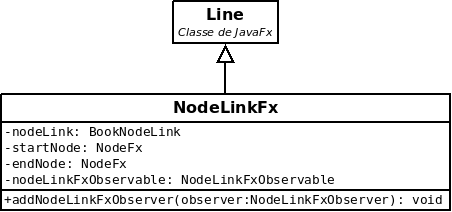
\includegraphics[width=0.6\textwidth, keepaspectratio]{img/NodeLinkFx.png}
					\caption{UML sur la représentation des liens}
				\end{figure}

				Comme on peut le voir, ceux ci héritent de la classe \textbf{Line}. De la même manière que \textbf{NodeFx}, la classea comme attribut l'objet qu'elle représente, c'est à dire une instance de \textbf{BookNodeLink}. On va également retrouver le noeud de départ et de fin ce qui permet de facilement connaitre ces noeuds lorsque l'on éditera le lien pour, par exemple, ajouter des champs supplémentaires si c'est un noeud de combat ou un noeud aléatoire.

				Voici quelques informations supplémentaire :

				\begin{itemize}
					\item{Il est important de noter que l'héritage fait avec les éléments de JavaFx permet d'ajouter nos classes comme on pourrait ajouter n'importe quel autre élément de cette librairie.}
					\item{L'utilisation du Pattern Observer est fait de tel manière que l'on puisse être notifié dès que l'on clique sur l'élément sans avoir besoin de passer par les évènements de JavaFx.}
				\end{itemize}

			\subsubsection{Gestion des évènements}

				On distingue l'écoute d'évènement à trois endroits. Sur la zone d'édition, sur un noeud et sur un lien.

				Sur la zone d'édition nous surveillons notamment les cliques lorsque nous somme en mode "ADD\_NODE". Dans le cas où un clique intervient, nous affichons la boite de dialogue permettant l'ajout d'un noeud puis, si nous avons validé cette dernière, nous ajoutons alors le noeud au livre. On recevra alors une "notification" grace à la méthode prévu à cet effet par le Pattern Observer que le noeud à été ajouté et qu'il faut donc l'afficher.

				Lorsque nous créons un noeud, nous devons faire en sorte qu'il réagisse avec les prochains évènement, de ce fait, nous ajoutons le \textbf{GraphPane} à la liste des observers du noeud. Dès lors, un clique sur ce noeud sera automatiquement perçue et traité dans la méthode correspondante.

				Afin de réaliser un lien entre les deux noeuds, il faut cliquer sur un noeud puis sur un second tout en ayant sélectionné le mode "ADD\_NODE\_LINK". On retient dans une variable le premier noeud cliqué. Lors d'un clique sur un noeud, cette variable prend alors la valeur de celui-ci et rien de plus ne se passe. Lorsque l'on cliquera de nouveau sur un noeud, alors, comme la variable ne vaut plus "null", on affichera la boite de dialogue permettant de remplir les informations sur le lien entre ces deux noeuds. Comme pour le noeud, si on valide la boiite de dialogue, alors on ajoute à la classe \textbf{Book} le lien et une "notification" est perçue par la méthode correspondante.

				De même, afin de recevoir les évènement concernant le lien, on enregistre le \textbf{GraphPane} comme étant observer de celui-ci. Cela nous permet maintenant de réagir par exemple à la demande de suppression d'un noeud.

		\subsection{RightPane}

			Ce panel contient toutes les statistiques concernant le livre. Celles-ci sont immédiatement mise à jour lorsqu'un élément du livre change grace, comme mentionné précedemment, au Pattern Observer.

			Pour le moment, les statistiques ne concernent que le nombre de noeuds de chaque type ainsi que la difficulté du livre. Dès qu'un noeud est ajouté, on incrémente les compteurs correspondant. De même, dès qu'un noeud se retrouve supprimé, on décrémente les compteurs qui doivent l'être. Un changement de livre reset les compteurs et, compte le nombre de noeud de chaque type. C'est le seul moment où l'on va parcourir tous les éléments du livre. En effet, le système de compteur permet de gagner un gain de temps sur des livres contenant de nombreux noeuds. Pour la difficulté du livre, il est possible de mettre à jour la valeur affiché avec la méthode \textit{void difficultyChanged(float)}. C'est notamment ce que l'on fait une fois que celle-ci à fini d'être calculée avec le menu \underline{Livre -> Estimer la difficulté}.

	\section{Rendre le livre jouable et estimer sa difficulté}
		\label{sec:Jeu}

		\subsection{Jeu}

			Une classe a été créée, se nommant \textbf{Jeu}, permettant de gérer les méthodes de jeu communes entre les classes \textit{Player} et \textit{Fourmis}. Cela permet donc d'avoir une classe qui gère tout le jeu en faisant appel aux différentes méthodes et classes en fonctions du types de noeud et du type de joueur. \\
			Un construteur est d'abord appelé, à partir de la MainWindow, afin d'envoyer le livre contenant toutes les informations. Puis, en fonction du mode sélectionner (\textbf{Générer la difficulté} ou \textbf{Jouer}), la méthode correspondante au joueur est appelé.\\

			Soit la méthode \textit{play()} est appelé si \textbf{Jouer} est sélectionné. C'est donc le player qui va jouer. Cela veut dire que les messages vont alors s'afficher dans le terminal (\textit{showMessages}) et le player est défini sur la classe \textit{Player}. Cela permetra d'appeler le bon joueur lors de l'appélation des méthodes où un choix est nécessaires.
			Une fois le jeu lancer grâce au \textit{runGame()}, expliqué dans le code \ref{lst:runGame} et les ressources temporaires qui ont été généré sont supprimés.

			\begin{lstlisting}[gobble=16, language=java, caption=play()]
				public void play() throws IOException, BookFileException {
					player = new Player();

					showMessages = true;

					runGame();

					cleanUp();
				}
			\end{lstlisting}

			Soit la méthode \textit{fourmis()} est appelé si \textbf{Générer la difficulté} est sélectionné. Ce sont donc plusieurs fourmis qui vont jouer une par une afin de générer la difficulté du livre. Les messages sur le terminal sont donc non affiché. Puis vient le lancement des fourmis. Pour cela une boucle "for" est simplement necessaire. Le player est donc défini sur la classe \textbf{Fourmis} permettant ainsi d'utiliser les méthodes de cette classe afin de réaliser des choix random. Puis la méthode \textit{runGame()}, expliqué dans le code \ref{lst:runGame}, renvoi donc la finalité du livre: soit un boolean true en cas de victoire ou false en cas de défaite.\\
			On a donc une classe qui permet réaliser des choix random ainsi qu'une méthode qui renvoie la finalité du livre. Cela permet donc de lancer un certain nombre de "fourmis" qui vont parcourir tout le livre, réalisé des choix, gagner ou perdre. Toutes les victoires vont être comptés, ce qui va permettre de savoir combien de fourmis ont gagnés. Soit calculé la difficulté du livre.

			\begin{lstlisting}[gobble=16, language=java, caption=fourmis()]
				public float fourmis(int nbrFourmis) throws IOException, BookFileException {
				   showMessages = false;

				   int victoire = 0;
				   for(int i = 0 ; i < nbrFourmis ; i++){
					   player = new Fourmi();

					   if(runGame()) {
						   victoire++;
					   }
				   }

				   cleanUp();

				   return ((float)victoire / (float)nbrFourmis) * 100f;
				}
			\end{lstlisting}

			Une fois dans la méthode choisis, la méthode \textit{runGame()} est alors appelé. C'est la méthode principal de la classe \textbf{Jeu} car c'est elle qui lance le jeu.
			Tout d'abord, la méthode copie le livre afin de ne pas le modifier par erreur pendant le jeu. Car même si on a fait attention, il suffit d'une erreur pour modifier tout le livre principal qui gère le jeu. Puis un BookState, qui correspond à l'état de la partie, est créé. Ce BookState permettera donc de suivre l'état du livre ainsi que du joueur (son inventaire, sa santé...). D'ailleur, le joueur enregistré dans le BookState est soit le personnage principal créer dans le prélude, soit, si inexistant, un personnage prééxistant permettant ainsi de jouer au jeu sans pour autant créer un personnage principal (voir méthode si dessous). Enfin, si des compétences et/ou des items sont disponible au début de la partie, la méthode de création de joueur (\textit{execPlayerCreation}, voir \ref{lst:execPlayerCreation}) est appelé en fonction du joueur actuel.

			\begin{lstlisting}[gobble=16, language=java, caption=createNewState()]
				BookCharacter bookCharacter;
				BookState newState = new BookState();

				if(this.book.getMainCharacter() == null){
					//Création d'un personnage
				}
				else {
					//Récupération du personnage principal
				}

				//Affichage pour le joueur du personnages principal

				newState.setBook(this.book);

				//Conception du personnage (ajout de compétences, items)

				return newState;
			\end{lstlisting}

			Une fois le \textbf{BookState} créé, le personnage principal initialisé et la copie du livre enregistré, le premier noeud est donc chargé. La boucle while du \textit{runGame()} est donc lancé et ne s'arrètera qu'une fois la partie terminée. Comme vous pouvez le remarquer, sur le code ci-dessous, chaque méthode correspond à un type de noeud en particulier. Les méthodes s'exécutent alors, puis renvoie le noeud de destination, en fonction du choix du joueur et / ou de la mort du joueur. Durant l'exécution des différentes méthodes et en fonction du joueur, d'autres méthodes externe sont appelées nottament dans la classe \textbf{Fourmis} ou \textbf{Player}. Tout ceci permet de minimiser le code en commun.

			\begin{lstlisting}[gobble=16, language=java, label=lst:runGame, caption=Méthode runGame()]
				while(!gameFinish){
					if(currentNode instanceof BookNodeCombat){
						//execNodeCombat(bookNodeCombat);
					}
					else if(currentNode instanceof BookNodeWithChoices){
						//execNodeWithChoices(bookNodeWithChoices);
					}
					else if(currentNode instanceof BookNodeWithRandomChoices){
						//execNodeWithRandomChoices(bookNodeWithRandomChoices);
					}
					else if(currentNode instanceof BookNodeTerminal){
						//execNodeTerminal(bookNodeTerminal);
						//Si partie gagné, win = true
					} else {
						//BookNodeTerminal FAILURE
					}
				}
				return win;
			\end{lstlisting}

			Pour chaque type de noeud, sauf pour un noeud terminal car il ne contient pas ces options, une méthode commune, nommé \textit{execAbstractNodeWithChoices()} est appelé afin de savoir si le noeud pris en charge fait gagné/perdre de la vie (méthode \textit{execNodeHp()}), puis regarde si le joueur est toujours en vie. Cela permet donc que chaque exécution de noeud vérifie ceci, permettant ainsi de minimisé la redondance. Si le joueur n'est plus en vie, un noeud terminal de défaite est alors renvoyé en noeud de destination, permettant ainsi de notifier la défaite du joueur. S'il est encore en vie et que le noeud propose des items, ils sont proposés au joueur en appelant la méthode correspondante entre \textbf{Fourmis} ou \textbf{Player}. Ces classes sont appelé car le player doit faire un choix grâce au Scanner et la fourmis doit effectuer un choix random.\\

			\begin{lstlisting}[gobble=12, language=java, caption=Méthode execAbstractNodeWithChoices(), label=lst:execAbstractNodeWithChoices]
				public AbstractBookNode execAbstractNodeWithChoices(AbstractBookNodeWithChoices node){
					//Affichage pour le joueur

					execNodeHp(node);

					if(!state.getMainCharacter().isAlive()){
						//Création du noeud terminal de défaite
						return nodeTerminal;
					}

					if(!node.getItemLinks().isEmpty())
						chooseItems(node);

					return null;
				}
			\end{lstlisting}

			Puis, à chaque destination du joueur, sauf si celui ci a été entrainé vers un noeud terminal de défaite créer par la classe jeu et donc, non existante, une autre méthode est appelé (nommé \textit{execBookNodeLink()}) afin de regarder si le lien entre le noeud de départ et de destination fait perdre ou gagner de la vie et/ou de l'argent. Si c'est le cas, le joueur est alors "mis à jour". Si le joueur n'a plus de vie, même si le lien le portait vers un noeud de victoire, un noeud de défaite est créé. Le joueur est considéré alors comme perdant. Cela permet donc d'avoir une méthode complète pour la gestion des options dans les liens.

			\textbf{Si un noeud est de type basic}, il est alors pris en charge dans la méthode \textit{execNodeWithChoices()}, comme vous pouvez le constater dans la figure \ref{fig:JeuBookNodeWithChoices}. La méthode vérifie si au moins un choix est possible, pemettant ainsi de créer, ou non, un noeud terminal de défaite. S'il peut au moins choisir une destination, un choix est demandé parmis toutes les destinations faisant un appel à la méthode en fonction du joueur (\textit{player.makeAchoice()}). Car ici, un choix est demandé, soit le Scanner du player ou le random de la fourmis. Une fois le choix décidé, si le joueur a les prérequis pour aller vers cette destination (si \textit{isAvailable()} renvoie true), alors la méthode \textit{execBookNodeLink()}, vu juste en dessous de la figure du haut, est appelé. Si le joueur est toujours en vie, le noeud choisi est renvoyé en noeud de destination. Sinon, le joueur doit faire un autre choix car il y a minimum un choix possible.\\

			\begin{figure}[H]
				\centering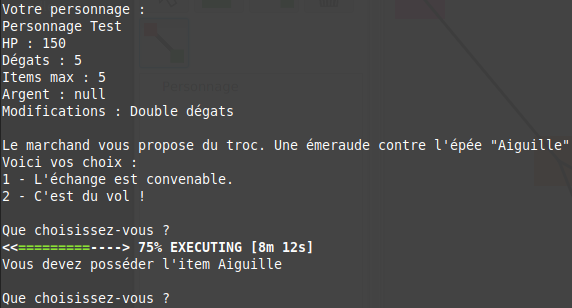
\includegraphics[width=0.70\textwidth]{img/codeJeuPrerequis.png}
				\caption{Jeu prérequis}
				\label{fig:codeJeuPrerequis}
			\end{figure}

			Le problème de la méthode \textit{isAvailable()}, c'est que cela peut créer un livre sans fin. En effet, prenons l'exemple d'un joueur avec un espace inventaire maximal de 1. Le joueur a un item, dans le premier noeud, "Potion" et décide de prendre l'item. Il n'a donc plus de place dans son inventaire. Le deuxième noeud, il décide de prendre l'item "Arme" car il veut pouvoir se défendre, l'item "Potion" est donc supprimé. Sauf qu'il se retouve en face de deux choix: Choix 1 avec de prérequi "Potion" qu'il vient de suprimmer, ainsi que le choix 2 qui le renvoi sur ce noeud. Le problème c'est que la méthode \textit{isAvailable()} renvoie true, car le joueur peut accéder au choix 2. Le joueur est donc coincé. Cela pose un problème que cela soit dans la génération de la difficulté et la jouabilité du livre.\\
			Cela ouvre donc une piste de réflexion. Il faudrait peut être envoyer des fourmis à chaque "destination" de noeud trouvé. Si une fourmis trouve une boucle infini (retombe sur un même noeud "n" fois, avec un nombre assez grand permettant d'être sûr que c'est bien une boucle infini), elle renvoie un "false" et le numéro du noeud. Si le joueur tombe sur ce paragraphe, un noeud terminal défaite est généré en indiquant sur celui ci "le livre n'est plus possible, il vous manque [prerequi]". Ces fourmis et ce boolean sera généré a chaque destination chargé. La fourmis sera la copie exacte du personnage au moment même du chargement du noeud de destination. Mais cette méthode ralentirais l'application et une autre, plus simple, serait peut être possible.

			\begin{figure}[H]
				\centering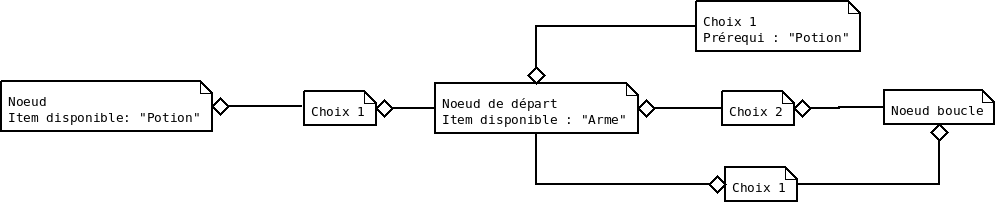
\includegraphics[width=0.70\textwidth]{img/JeuBoucleInfiniExemple.png}
				\caption{Exemple de boucle infini}
			\end{figure}


			Une fois qu'au moins une destination est possible, nous avons décidé de ne pas afficher que les choix possibles afin de ne pas aveugler le joueur de ses possibilités. S'il veut rejouer au livre, il saura les prérequis de certain chemins.

			\begin{figure}[H]
				\centering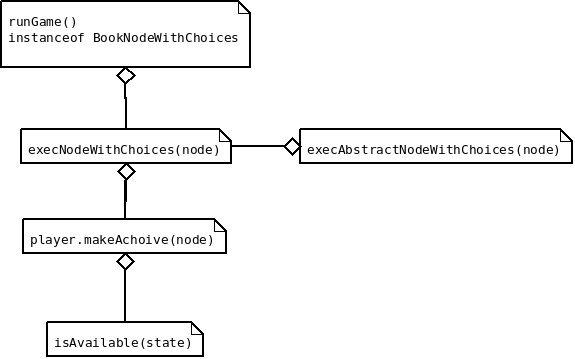
\includegraphics[width=0.70\textwidth]{img/JeuBookNodeWithChoices.png}
				\caption{Lien entre les méthodes pour un noeud basique}
				\label{fig:JeuBookNodeWithChoices}
			\end{figure}


			\textbf{Si c'est un noeud de type combat}, une vérification est réalisé afin savoir si le noeud contient des ennemis. S'il n'y a pas d'ennemis, le noeud en cas de victoire est envoyé en noeud de destination. S'il ny a pas de noeud de victoire, un noeud de défaite est automatiquement transmit afin de ne pas avoir d'erreur sur ce noeud. Si une liste d'ennemis est présente, cette dernière est copié est créé afin de ne pas modifier la vie des ennemis. Car ces derniers ne sont pas lié au noeud, mais c'est l'ID de l'ennemi qui est lié au noeud. Cela permet donc de les appelés plusieurs fois dans plusieurs ou dans le même noeud.\\
			Le combat commence alors. Le choix est défini par la méthode du joueur correspondant car un Scanner ou un random est requis pour ce type de choix. Ici, trois choix sont possibles:

			\begin{description}
				\item[Choix Attaque :]{que ce soit dans la classe \textbf{Player} ou \textbf{Fourmis}, un autre choix (cf ligne 2) est demandé permettant de sélectionner l'ennemi à attaquer parmi la liste des ennemis encore en vie. Cela permet donc de créer un dynamisme et une certaine intélligence dans le combat. Je vous invite à voir les subsection fourmis \ref{sub:fourmis} et player \ref{sub:player} pour plus de détail dans le choix.
				 Une fois l'ennemi sélectionné, une méthode attaque (cf ligne 7) est appelé apellant elle même une autre méthode commune entre l'attaque du joueur et l'attaque d'ennemi. Nommé \textit{getDamageAmount()}, elle permet de savoir le nombre de dommage réalisé en fonction des point d'attaque de l'attaquant, de son double dommage décider en random si ce boolean est défini en true, d'un coup critique décider aussi en random, de l'arme de l'attaquant et de l'item de défense de l'attaqué. L'attaquant et l'attaqué est défini en fonction de la permière méthode qui l'appel. Ici c'est la méthode d'attaque du player. Cette méthode commune permet donc d'éviter une répétition dans le code.}
				Une fois l'attaque effectué, si l'ennemi attaqué est mort, il est supprimé de la liste des ennemis (cv logne 9) avant sont tour pour éviter que l'ennemi mort attaque ou que l'on rattaque cette ennemi.
				\item[Inventaire :]{si ce choix est fait par le joueur, la méthode appelé permettant d'utiliser son inventaire est elle même gérer dans la classe Player ou la classe Fourmis. Elle permet alors de choisir une potion, une arme et ou un item de défense. Pour plus de détail sur ce choix, je vous invite à regarder les subsection fourmis \ref{sub:fourmis} et player \ref{sub:player}.}
				\item[Evasion :]{si le tour avant évasion est inférieur ou égal à 0 (voir cf 13) et si un noeud de d'évasion existe, le joueur peut alors s'enfuir. Sinon cela lui passe son tour.Nous avons décidé de ne pas relancer les choix à ce moment, car cela peut être une stratégie du joueur qui, dans une prochaine mise à jour d'implentation de pouvoir lié à des compétences, en cas d'une compétence de "renvoi" (qui se désactive en cas d'attaque de la part du joueur), l'attaque de l'ennemi est alors "retourné" vers lui même.}
			\end{description}

			\begin{lstlisting}[gobble=16, language=java, caption=JeuCombat]
				while(!finCombat){
					ChoixCombat choixCombat = player.combatChoice(node, evasionRound, state);

					if (choixCombat == ChoixCombat.ATTAQUER) {

						BookCharacter ennemi = player.chooseEnnemi(listEnnemis);
						attaque(ennemi);
						if(!ennemi.isAlive()){
							listEnnemis.remove(ennemi);
						}
					}
					else if(choixCombat == ChoixCombat.EVASION) {
						if(evasionRound <= 0 && node.getEvasionBookNodeLink() != null){
							execBookNodeLink(node.getEvasionBookNodeLink());
							return book.getNodes().get(node.getEvasionBookNodeLink().getDestination());
						}
					}

					ennemiTour(listEnnemis);

					if(!state.getMainCharacter().isAlive()) {
						//Vérification d'un noeud Failure
						if(node.getLooseBookNodeLink() != null)  {
							execBookNodeLink(node.getLooseBookNodeLink());
							return book.getNodes().get(node.getLooseBookNodeLink().getDestination());
						} else
							return new BookNodeTerminal("Vous succombez à vos blessures", BookNodeStatus.FAILURE);
					}

					if(listEnnemis.isEmpty())
						finCombat = true;

					evasionRound -= 1;
				}
			\end{lstlisting}

			Une fois le tour du joueur fini, vient le tour de l'ennemi. Il appel une méthode envoyant la liste d'ennemis restant. Cette méthode appel \textit{getDamageAmount()} permettant aux ennemis d'attaquer un par un. Cette liste d'ennemis et la méthode commune, \textit{getDamageAmount()}, est alors très pratique pour l'attaque de l'ennemis et est, on pense, le meilleur moyen utiliser afin de gérer les attaques.\\

			La fin de combat est déterminé si la liste d'ennemis est vide ou si le joueur n'est plus en vie. Le noeud de destination est alors défini en fonction du résultat en fin de combat. Bien sur, si le noeud de destination n'est pas existant, la noeud terminal de défaite est créer pour éviter de bloquer le jeu.

			\textbf{Si le noeud est de type aléatoire}, la méthode commune est appelé afin de savoir si le joueur est encore en vie. Puis une autre méthode, nommé \textit{getRandomChoices()} (cf \nameref{lst:getRandomChoices} à la page \pageref{lst:getRandomChoices}) est appelé de la classe BookNodeLinkRandom afin de déterminer le noeud de destination en fonction des chances attribué à chacun de ces choix.

			\textbf{Si le noeud est de type terminal}, la partie est alors terminé et renvoie un boolean sur l'état de la fin de partie. Ce boolean permet de quitter la boucle while de la méthode \textit{runGame()} et permet ainsi donc d'arreter le jeu. L'utilisateur peut alors continuer l'édition du livre pour le player et permet de savoir si la partie est gagné ou perdu pour la fourmis (voir la subsection fourmis \ref{sub:fourmis}). Bien sûr, une vérification si le joueur est en vie est également éxécuté si c'est une noeud de type VICTORY, permettant ainsi que le joueur perde même si le son lieu de destination est un noeud de victoire.

		\subsection{Interface Player / Foumis}
			Une interface \textbf{InterfacePlayerFoumis} a été créé permettant une mise en commun des codes \textbf{Player} et \textbf{Fourmis}. Ces méthodes permettent de faire un choix, prendre les items disponibles, créer un personage lambda, aller dans l'inventaire, choisir son ennemis ou encore combatre. Elles sont appelé au même moment. La méthode sera alors exécuté différément en fonction du joueur. Ce sont des méthode communes car un choix est demandé, et la décision du choix est différentes en fonction d'un joueur ou d'une fourmis. En effet, un Scanner est utilisé afin de prendre en compte le choix du player et un nombre aléatoire est généré pour la fourmis.

			Ci-dessous, toutes les méthodes communes sont présentés de façon général. Mais elles seront toutes expliquer dans les subsection fourmis \ref{sub:fourmis} et player\ref{sub:player}, vu un peu plus bas.

			\textit{execPlayerCreation} permet de choisir les compétences et les items disponibles au début de la partie. Ces derniers sont défini lors de la création du prélude. Pour l'ajout des items, la méthode \textit{prendItems} est appelé. Cette méthode permet donc de jouer au livre avec peut être, différentes finalités en fonction de ces choix.

			\textit{combatChoice}, prend en paramètre le noeud de Combat et le nombre de tour avant l'évasion ainsi que le BookState. Elle permet de faire un choix lors du tour du joueur dans un combat. On peut alors choisir d'attaquer, d'aller dans l'inventaire ou alors de s'évader. Si on choisi l'inventaire, on va alors dans une autre méthode appelé \textit{useInventaire} qui prend le BookState en paramètre. On peut alors utiliser un item de santé, prendre un objet de défense ou alors une arme. Si l'on choisis un autre choix, cette objet n'est pas utilisable lors d'un combat (comme par exemple de l'argent). Une fois l'objet pris, on retourne dans les choix du combat. On peut alors, soit retourner dans l'inventaire pour prendre un autre objet, soit attaquer ou s'évader. Cela donne donc libre choix au joueur sur le nombre d'objet à utiliser (comme par exemple, l'ajout d'une arme ainsi qu'un bouclier).

			\textit{chooseEnnemi} permet de choisir l'ennemi à attaquer parmi la liste de tout les ennemis encore en vie. Cela rend le système de combat un peu plus "intelligent".

			\textit{prendItems} permet de prendre un item parmi la liste d'items disponible. Cette liste est pris en paramètre ainsi que la sauvegarde de la partie et le nombre d'item maximum pouvant être pris. Cela permet ainsi d'avoir une méthode complète qui peut être utiliser pour prendre les items disponibles aux prélude comme sur les différents noeuds du livre.

			\textit{makeAChoice} permet de faire un choix en fonction des différentes destinations proposé par le noeud. Cette méthode est ce qui défini un "livre à choix".

			\textit{useIventaire} permet d'utiliser son inventaire lors d'un noeud de combat. La mise à jour d'un port d'item de défense ou d'arme est alors mis à jour. Si un item de soin est choisi, les points de vie du joueur sont alors actualisée.

			Malgré une séparation entre le code en "communs" visible dans la classe \textbf{Jeu} et le code normalement "non communs" visible dans les classes \textbf{Player} et \textbf{Fourmis}, vous allez remarquer dans l'explication de ses classes, qu'une partie est encore commune. Ce problème n'a pas été réglé par manque de temps.

		\subsection{Player}\label{sub:player}
			La classe \textbf{Player} permet de jouer au jeu en tant que player. Elle permet de faire des choix grâce aux Scanner permettant ainsi l'avancement du jeu. Des messages sont aussi affiché afin de guider le player dans ses choix.\\
			Nottament la méthode \textit{choixYesNo()} qui permet de choisir Oui ou Non et de renvoyer le boolean true ou false. Cette méthode permet, par exemple, de savoir si le player veut supprimer, prendre un item ou une compétence. Elle a donc été créé évitant ainsi la redondance de code.\\

			Pour la méthode commune \textit{prendItems()}, cette dernière fait appel à d'autre méthodes présente dans la classe \textbf{Player}.

			\begin{lstlisting}[gobble=16, language=java, label=lst:prendreItemsPlayer, caption=prendreItems() du Player]
				public void prendreItems(BookState state, List<BookItemLink> bookItemLinks, int nbItemMax){
					while(nbItemMax != 0 && !bookItemLinks.isEmpty()){
						System.out.println("Les items suivant sont disponible:");
						//Affiche les items

						System.out.println("Voulez vous un item ?");
						if(choixYesNo()){
							int itemMax = state.getMainCharacter().getItemsMax();

							if(itemMax == state.getMainCharacter().getItems().size()){
								itemPlein(state);

								System.out.println("Voici vos choix:");

								if(choixYesNo())
									nbItemMax = 0;
								else
									itemSupp(state);
							} else {
								itemAdd(state, bookItemLinks);
							}

						} else {
							nbItemMax = 0;
						}

						if(bookItemLinks.isEmpty())
							nbItemMax = 0;
					}
				}

			\end{lstlisting}

			Par exemple, \textit{itemAdd()} (cf ligne 20 dans le code \ref{lst:prendreItemsPlayer}) qui elle permet de choisir l'item à ajouter dans l'inventaire. Une variable "choixValide" permet de ne pas valider un numéro de choix non valide. Une fois l'item choisi, l'ID de l'item est alors ajouter dans la liste de l'inventaire afin de pouvoir retrouver l'item si le joueur l'utilise.\\
			Cette méthode a été créé permettant de séparer le code de la méthode \textit{prendItems()} pour une meilleure visibilité. Elle pourrait aussi servir, par exemple, dans l'ajout d'un item obligatoire. Dans ce cas, la méthode \textit{prendItems()} n'est plus utilisé mais directement \textit{itemAdd()}. Mais cette exemple n'est pas représentatif de l'état actuel de MagicBook qui ne permet pas de rendre un item obligatoire. Mais c'est une idée d'amélioration.\\

			\begin{lstlisting}[gobble=16, language=java, caption=itemAdd()]
				private void itemAdd(BookState state, List<BookItemLink> bookItemLinks){
					System.out.println("Quel item voulez-vous ?");
					boolean choixValide = false;
					int choix = -1;

					while(!choixValide){
						Scanner scanner = new Scanner(System.in);
						choix = scanner.nextInt();

						if(choix >= 0 && choix <= (bookItemLinks.size()-1)){
							choixValide = true;
						} else {
							System.out.println("vous ne pouvez pas effectuer ce choix");
						}
					}

					BookItemLink itemLink = bookItemLinks.get(choix);
					System.out.println("L'item "+state.getBook().getItems().get(itemLink.getId()).getName()+" a été rajouté");
					state.getMainCharacter().getItems().add(itemLink.getId());

					itemLink.setAmount(itemLink.getAmount()-1);

					if(itemLink.getAmount() == 0)
						bookItemLinks.remove(itemLink);
				}

			\end{lstlisting}

			Puis la méthode \textit{itemPlein()} (cf ligne 11 dans le code \ref{lst:prendreItemsPlayer}), qui elle, affiche les items à supprimer. Cette méthode permet d'afficher les items de l'inventaire.

			\begin{lstlisting}[gobble=16, language=java, caption=itemPlein()]
				private void itemPlein(BookState state){
					System.out.println("Votre inventaire est plein");
					System.out.println("Voulez vous supprimer un item ?");
					System.out.println("Vos Item: ");

					int i = 0;
					for(String itemState : state.getMainCharacter().getItems()){
						System.out.println(i + " - "+state.getBook().getItems().get(itemState));
						i++;
					}
				}
			\end{lstlisting}

			Pour la méthode \textit{itemSupp}, elle est appelé (cf ligne 18 dans le code \ref{lst:prendreItemsPlayer}) afin de choisir l'item à supprimer. Une boucle while est alors parcouru afin d'être sûr d'avoir un choix valide. Une fois l'item choisi, cela met l'inventaire du player à jour grâce au state pris en charge dans la méthode \textit{prendreItems}. Bien sûr, l'utilisateur à le choix de ne pas supprimer un item permettant ainsi de garder tout les items de son inventaire.
			On aurait pu très bien laisser le choix au player de supprimer quand même un item si son inventaire n'était pas plein. Mais c'est un livre à choix avec des prérequis, tout les items peuvent donc être important, et il n'y a pas de pénalité de déplacement si l'inventaire est plein. Cette fonctionalité de supprimer un item dans l'inventaire n'a alors pas été jugé nécessaire à ajouter en option libre.

			\begin{lstlisting}[gobble=16, language=java, caption=itemSupp()]
				private void itemSupp(BookState state){
					System.out.println("Quel item voulez-vous supprimer ?");
					boolean choixValide = false;

					while(!choixValide){
						Scanner scanner = new Scanner(System.in);
						int choix = scanner.nextInt();

						if(choix >= 0 && choix <= (state.getMainCharacter().getItems().size()-1)){
							state.getMainCharacter().getItems().remove(choix);
							choixValide = true;
						} else if(choix == -1) {
							choixValide = true;
						} else {
							System.out.println("vous ne pouvez pas effectuer ce choix");
						}
					}

				}
			\end{lstlisting}

			Pour la méthode \textit{itemAdd()}, elle permet d'ajouté un item choisi.
			Tout ceci est donc gérer par la méthode \textit{prendreItemsPlayer}, permettant ainsi d'appeler certaine méthode en fonction des choix du player ainsi que de gérer la prise des items grâce à la boucle while.


			Pour la méthode \textit{execPlayerCreation()} est presque la même que celle de la fourmis : elle utilise aussi la méthode \textit{prendItems()}, défini ici\ref{lst:prendreItemsPlayer} au moment de l'ajout des items. Mais au moment de l'ajout de compétences, la méthode \textit{skillAdd()} est appelé jusqu'à ce que le maximum de compétences autorisé a été pris ou qu'il n'en reste plus à prendre. Cette méthode ressemble fortement à la prise d'item. \textit{execPlayerCreation()} serais à implenté dans la classe \textit{Jeu}, car beaucoup de code est en commun.\\

			\begin{lstlisting}[gobble=16, language=java, caption=execPlayerCreation() du Player]
				public void execPlayerCreation(Book book, AbstractCharacterCreation characterCreation, BookState state){
					//Affichage du texte du début dans "création du personnage"

					if(characterCreation instanceof CharacterCreationItem){
						CharacterCreationItem characterCreationItem = (CharacterCreationItem) characterCreation;
						prendreItems(state, characterCreationItem.getItemLinks(), characterCreationItem.getAmountToPick());
					}
					else if(characterCreation instanceof CharacterCreationSkill){
						CharacterCreationSkill characterCreationSkill = (CharacterCreationSkill) characterCreation;

						int nbItemMax = characterCreationSkill.getAmountToPick();

						while(nbItemMax != 0 && !characterCreationSkill.getSkillLinks().isEmpty()){
							System.out.println("Les compétences suivant sont disponible:");
							//Affichage des compétences
							}

							skillAdd(state, characterCreationSkill);
							nbItemMax--;
						}
					}
				}
				\end{lstlisting}


		\subsection{Fourmis}\label{sub:fourmis}
			La classe \textbf{Fourmis} permet de parcourir le livre en tant que joueur fictif. Elle effectue des choix random en fonction des différentes méthodes de l'interface. Cela permet donc de terminer le livre grâce aux choix random.

			La méthode \textit{combatChoice} permet de choisir entre ATTAQUE, EVASION, INVENTAIRE. Nous avons choisi de faire un random sur les trois choix et non pas sur deux choix même si le tour d'évasion n'est pas disponible, permettant ainsi d'avoir la possibilité que la fourmi passe aussi son tour, comme le joueur, afin d'avoir la même chance lors des combats. Elle peut aussi utiliser son inventaire lors du combat.

			\begin{lstlisting}[gobble=16, language=java, caption=combatChoice() de Fourmis]
				public ChoixCombat combatChoice(BookNodeCombat bookNodeCombat, int remainingRoundBeforeEvasion, BookState state) {
					boolean choixValide = false;
					Random random = new Random();
					ChoixCombat choixCombat = null;
					int choix;

					while(!choixValide){
						choix = random.nextInt(ChoixCombat.values().length);
						choixCombat = ChoixCombat.values()[choix];

						if (choixCombat == ChoixCombat.INVENTAIRE){
							if(!state.getMainCharacter().getItems().isEmpty())
								useInventaire(state);
						} else {
							choixValide = true;
						}
					}

					return choixCombat;
				}
			\end{lstlisting}

			 Ainsi, elle peut se soigner, prendre des armes et/ou des items de défense. Malheureusement, la foumis n'est pas "intelligente" et ne prend pas donc la meilleur arme ou ne se soigne pas alors qu'elle va mourir. Mais c'est un gros point à améliorer. Elle choisi donc au hasard un des items et peut même prendre un items non utile dans le combat. Elle revient donc sur les trois choix ATTAQUE, EVASION, INVENTAIRE sans avoir pris une arme ou autre lors du choix de l'item dans son inventaire.

			\begin{lstlisting}[gobble=16, language=java, caption=useInventaire() de Fourmis]
				public void useInventaire(BookState state){
					List<String> listItemState = state.getMainCharacter().getItems();

					Random random = new Random();
					int choix = random.nextInt(listItemState.size());
					BookItem bookItem = state.getBook().getItems().get(listItemState.get(choix));

					if(bookItem instanceof BookItemDefense){
						state.setBookItemDefense((BookItemDefense) bookItem);
					}
					else if(bookItem instanceof BookItemHealing){
						BookItemHealing bookItemHealing = (BookItemHealing) bookItem;
						state.getMainCharacter().heal(bookItemHealing.getHp());
						state.getMainCharacter().getItems().remove(listItemState.get(choix));
					}
					else if(bookItem instanceof BookItemWeapon){
						state.setBookItemArme((BookItemWeapon) bookItem);
					}
				}
			\end{lstlisting}

			Autre point, lors de l'utilisation de la méthode \textit{prendreItems()}, la fourmis prend tout les items disponible, tant qu'elle a encore de la place, que le maximum d'objet à prendre n'est pas à 0 et si des objets sont encore disponible.

			\begin{lstlisting}[gobble=16, language=java, caption=prendreItems() de Fourmis]
				public void prendreItems(BookState state, List<BookItemLink> bookItemLinks, int nbItemMax){
					int choix = 0;

					while(nbItemMax != 0){
						int itemMax = state.getMainCharacter().getItemsMax();
						//Vérifie item maximum et si il y a encore des items à prendre
						if(state.getMainCharacter().getItems().size() < itemMax && !bookItemLinks.isEmpty()){
							//Choix
							Random random = new Random();
							choix = random.nextInt(bookItemLinks.size());

							BookItemLink itemLink = bookItemLinks.get(choix);

							state.getMainCharacter().addItem(itemLink.getId());
							itemLink.setAmount(itemLink.getAmount()-1);

							if(itemLink.getAmount() == 0)
								bookItemLinks.remove(itemLink);

							if(nbItemMax != -1)
								nbItemMax--;
						} else {
							nbItemMax = 0;
						}
					}
				}
			\end{lstlisting}

			Des boucles infini sont donc à prévoir si par exemple, un objet est requis pour accéder au choix 2 et qu'il faut aller dans le choix 1 pour prendre l'item. Vu qu'au moins un choix est disponible, aucun noeud terminal n'est généré. Sauf que si l'item de la fourmis est plein, l'item ne peut pas être pris et aucun item est supprimé. Si la supression est active, quel est l'item à suprimmer ? Comment définir un item important ? A la santé du personnage, au nombre d'objet non possédé d'un certain type (exemple: defense) ? A un nombre "d'importance" prédéfini à l'édition du livre ? Cette piste de réflexion serait donc à exploiter dans les améliorations à apporter.

			\begin{figure}[H]
				\centering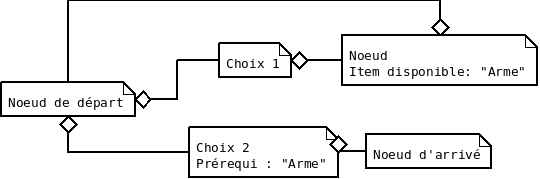
\includegraphics[height=2.5cm, keepaspectratio]{img/fourmisPrendreItemInfiniExemple.png}
				\caption{prendreItem exemple de boucle infini}
			\end{figure}[H]

			A la méthode \textit{execPlayerCreation()}, soit, à la création du personnage, le même problème se pose. En effet, la méthode \textit{prendreItems()} est utilisé. Pour l'ajout de compétence, le problème est moins important. En effet, les compétences ne peuvent pas être aprise autre part qu'à la création du personnage. En effet, c'est une autre amélioration prévu. Nous avons donc décidé d'ajouter le nombre maximal de compétence. Mais si les compétences avait des effets, comment définir qu'une compétence est plus importante qu'une autre ? Peur être avoir aussi un nombre prédéfini, comme les items, qui désigne son importance. Puis copier la méthode pour choisir un noeud aléatoire. Il faudrait aditionner tout les nombres désignant l'importance, choisir un nombre aléatoire, puis soustraire chaque nombres désignant l'importance jusqu'à être égal ou inférieur à zero. Ces une piste de réflexion possible, mais pas la seule solution.

			\begin{lstlisting}[gobble=16, language=java, caption=execPlayerCreation() de Fourmis]
				public void execPlayerCreation(Book book, AbstractCharacterCreation characterCreation, BookState state) {

					if(characterCreation instanceof CharacterCreationItem){
						CharacterCreationItem characterCreationItem = (CharacterCreationItem) characterCreation;

						prendreItems(state, characterCreationItem.getItemLinks(), characterCreationItem.getAmountToPick());
					}
					else if(characterCreation instanceof CharacterCreationSkill){
						CharacterCreationSkill characterCreationSkill = (CharacterCreationSkill) characterCreation;

						Random random = new Random();
						int amountToPick = characterCreationSkill.getAmountToPick();
						while(amountToPick != 0 && !characterCreationSkill.getSkillLinks().isEmpty()) {
							int choix = random.nextInt(characterCreationSkill.getSkillLinks().size());
							state.getMainCharacter().addSkill(characterCreationSkill.getSkillLinks().get(choix));
							characterCreationSkill.getSkillLinks().remove(choix);
							amountToPick--;
						}
					}
				}
			\end{lstlisting}

			Pour la méthode \textit{chooseEnnemi}, la fourmi envoyé prend obligatoirement le premier ennemi permettant de tuer le maximum d'ennemis en attaquant toujours le même ennemi. Nous avons choisi cette solution pour éviter que la fourmi attaque tout les ennemis sans en tuer un seul. Sauf qu'à chaque tour, chaque ennemi attaque. Donc moins il y a d'ennemis, plus sont les chances de remporter le combat.\\
			Mais un autre problème se pose. Imaginons une fourmi avec 15 points de vie 10 points d'attaque. Imaginons une liste ennemis: [20pts,5pts,5pts,5pts]. Si le premier ennemi à 20 point de vie et les troix suivant ont 5 points de vie, serait-il plus judicieux alors de tuer les troix ennemis avec 5 points de vie avant d'attaquer le premier ennemis avec 20 points de vie. Probablement oui. Voyons le problème de plus près.
			\begin{itemize}
				\item Attaque de la fourmis: deuxième de la liste
				\item Reste liste ennemis: [20pts,5pts,5pts]
				\item Attaque des ennemis: Le premier ennemi attaque (-5 points de vie à la fourmi, soit 10pts vie restant), les autres attaque aussi (-0pts de vie à la fourmi, soit 10pts vie restant)
			\end{itemize}

			En tant que player, il changerait d'ennemis. La fourmi devra alors avoir l'intelligence de changer d'adversaire. Elle gagnera alors de combat.

			\begin{itemize}
				\item Attaque de la fourmis: premier de la liste
				\item Perte de 10pts de vie sur le premier ennemi
				\item Reste liste ennemis: [10pts,5pts,5pts]
				\item Attaque des ennemis: Le premier ennemi attaque (-5 points de vie à la fourmi, soit 5pts vie restant), les autres attaque aussi (-0pts de vie à la fourmi, soit 5pts vie restant)
				\item Attaque de la fourmis: premier de la liste
				\item Reste liste ennemis: [5pts,5pts]
				\item Attaque des ennemis: les autres attaque aussi (-0pts de vie à la fourmi, soit 5pts vie restant)
				\item ...
			\end{itemize}
